\section{Modulação em Amplitude}
A modulação em amplitude (AM\abbrev{AM}{modulação em amplitude}, do inglês
\textit{Amplitude Modulation}) é o processo no qual a envoltória de uma onda
portadora oscila em torno de um valor médio, conforme um sinal modulador em
baixa frequência~\cite{haykin2008}. No contexto de telecomunicações, a
moduladora é um sinal em banda base, isto é, contém a informação em um espectro
delimitado a ser transmitida.

Considerando a portadora como um tom puro de frequência $f_c$ e amplitude $A_c$:
\symbl{$c(t)$}{portadora no domínio contínuo}
\symbl{$f_c$}{frequência da portadora}
\symbl{$A_c$}{amplitude da portadora}
\begin{equation}
    c(t) = A_c \cos(2\pi f_c t).
\end{equation}

    Um sinal $s(t)$ modulado em amplitude é definido pela composição de suas
parcelas portadora $c(t)$ e moduladora $m(t)$:
\symbl{$k_a$}{sensibilidade à amplitude}
\symbl{$m(t)$}{moduladora no domínio contínuo}
\symbl{$s(t)$}{sinal modulado no domínio contínuo}
\begin{figure}[H]
    \centering
    \resizebox{1.0\textwidth}{!}{%% Creator: Matplotlib, PGF backend
%%
%% To include the figure in your LaTeX document, write
%%   \input{<filename>.pgf}
%%
%% Make sure the required packages are loaded in your preamble
%%   \usepackage{pgf}
%%
%% Also ensure that all the required font packages are loaded; for instance,
%% the lmodern package is sometimes necessary when using math font.
%%   \usepackage{lmodern}
%%
%% Figures using additional raster images can only be included by \input if
%% they are in the same directory as the main LaTeX file. For loading figures
%% from other directories you can use the `import` package
%%   \usepackage{import}
%%
%% and then include the figures with
%%   \import{<path to file>}{<filename>.pgf}
%%
%% Matplotlib used the following preamble
%%
\begingroup%
\makeatletter%
\begin{pgfpicture}%
\pgfpathrectangle{\pgfpointorigin}{\pgfqpoint{18.000000in}{8.000000in}}%
\pgfusepath{use as bounding box, clip}%
\begin{pgfscope}%
\pgfsetbuttcap%
\pgfsetmiterjoin%
\pgfsetlinewidth{0.000000pt}%
\definecolor{currentstroke}{rgb}{1.000000,1.000000,1.000000}%
\pgfsetstrokecolor{currentstroke}%
\pgfsetstrokeopacity{0.000000}%
\pgfsetdash{}{0pt}%
\pgfpathmoveto{\pgfqpoint{0.000000in}{0.000000in}}%
\pgfpathlineto{\pgfqpoint{18.000000in}{0.000000in}}%
\pgfpathlineto{\pgfqpoint{18.000000in}{8.000000in}}%
\pgfpathlineto{\pgfqpoint{0.000000in}{8.000000in}}%
\pgfpathlineto{\pgfqpoint{0.000000in}{0.000000in}}%
\pgfpathclose%
\pgfusepath{}%
\end{pgfscope}%
\begin{pgfscope}%
\pgfpathrectangle{\pgfqpoint{2.250000in}{1.000000in}}{\pgfqpoint{4.102941in}{6.040000in}}%
\pgfusepath{clip}%
\pgfsetrectcap%
\pgfsetroundjoin%
\pgfsetlinewidth{0.752812pt}%
\definecolor{currentstroke}{rgb}{0.000000,0.000000,0.000000}%
\pgfsetstrokecolor{currentstroke}%
\pgfsetdash{}{0pt}%
\pgfpathmoveto{\pgfqpoint{2.250000in}{4.020000in}}%
\pgfpathlineto{\pgfqpoint{6.352941in}{4.020000in}}%
\pgfusepath{stroke}%
\end{pgfscope}%
\begin{pgfscope}%
\pgfpathrectangle{\pgfqpoint{2.250000in}{1.000000in}}{\pgfqpoint{4.102941in}{6.040000in}}%
\pgfusepath{clip}%
\pgfsetrectcap%
\pgfsetroundjoin%
\pgfsetlinewidth{0.752812pt}%
\definecolor{currentstroke}{rgb}{0.000000,0.000000,0.000000}%
\pgfsetstrokecolor{currentstroke}%
\pgfsetdash{}{0pt}%
\pgfpathmoveto{\pgfqpoint{2.436497in}{1.000000in}}%
\pgfpathlineto{\pgfqpoint{2.436497in}{7.040000in}}%
\pgfusepath{stroke}%
\end{pgfscope}%
\begin{pgfscope}%
\pgfpathrectangle{\pgfqpoint{2.250000in}{1.000000in}}{\pgfqpoint{4.102941in}{6.040000in}}%
\pgfusepath{clip}%
\pgfsetrectcap%
\pgfsetroundjoin%
\pgfsetlinewidth{1.505625pt}%
\definecolor{currentstroke}{rgb}{0.000000,0.000000,0.000000}%
\pgfsetstrokecolor{currentstroke}%
\pgfsetdash{}{0pt}%
\pgfpathmoveto{\pgfqpoint{2.436497in}{5.435625in}}%
\pgfpathlineto{\pgfqpoint{2.460509in}{5.434082in}}%
\pgfpathlineto{\pgfqpoint{2.484677in}{5.429422in}}%
\pgfpathlineto{\pgfqpoint{2.509311in}{5.421498in}}%
\pgfpathlineto{\pgfqpoint{2.534644in}{5.410063in}}%
\pgfpathlineto{\pgfqpoint{2.560987in}{5.394727in}}%
\pgfpathlineto{\pgfqpoint{2.588574in}{5.375033in}}%
\pgfpathlineto{\pgfqpoint{2.617792in}{5.350308in}}%
\pgfpathlineto{\pgfqpoint{2.649031in}{5.319739in}}%
\pgfpathlineto{\pgfqpoint{2.682834in}{5.282234in}}%
\pgfpathlineto{\pgfqpoint{2.719979in}{5.236284in}}%
\pgfpathlineto{\pgfqpoint{2.761864in}{5.179397in}}%
\pgfpathlineto{\pgfqpoint{2.811442in}{5.106615in}}%
\pgfpathlineto{\pgfqpoint{2.878971in}{5.001497in}}%
\pgfpathlineto{\pgfqpoint{3.008201in}{4.799597in}}%
\pgfpathlineto{\pgfqpoint{3.059023in}{4.726619in}}%
\pgfpathlineto{\pgfqpoint{3.101530in}{4.670822in}}%
\pgfpathlineto{\pgfqpoint{3.139063in}{4.626506in}}%
\pgfpathlineto{\pgfqpoint{3.173177in}{4.590881in}}%
\pgfpathlineto{\pgfqpoint{3.204649in}{4.562368in}}%
\pgfpathlineto{\pgfqpoint{3.234101in}{4.539764in}}%
\pgfpathlineto{\pgfqpoint{3.261843in}{4.522284in}}%
\pgfpathlineto{\pgfqpoint{3.288264in}{4.509217in}}%
\pgfpathlineto{\pgfqpoint{3.313675in}{4.500044in}}%
\pgfpathlineto{\pgfqpoint{3.338308in}{4.494393in}}%
\pgfpathlineto{\pgfqpoint{3.362476in}{4.491988in}}%
\pgfpathlineto{\pgfqpoint{3.386488in}{4.492695in}}%
\pgfpathlineto{\pgfqpoint{3.410578in}{4.496500in}}%
\pgfpathlineto{\pgfqpoint{3.435056in}{4.503518in}}%
\pgfpathlineto{\pgfqpoint{3.460156in}{4.513961in}}%
\pgfpathlineto{\pgfqpoint{3.486188in}{4.528187in}}%
\pgfpathlineto{\pgfqpoint{3.513464in}{4.546682in}}%
\pgfpathlineto{\pgfqpoint{3.542216in}{4.569985in}}%
\pgfpathlineto{\pgfqpoint{3.572911in}{4.598931in}}%
\pgfpathlineto{\pgfqpoint{3.605938in}{4.634419in}}%
\pgfpathlineto{\pgfqpoint{3.642072in}{4.677897in}}%
\pgfpathlineto{\pgfqpoint{3.682481in}{4.731495in}}%
\pgfpathlineto{\pgfqpoint{3.729495in}{4.799192in}}%
\pgfpathlineto{\pgfqpoint{3.789797in}{4.891808in}}%
\pgfpathlineto{\pgfqpoint{3.959591in}{5.155725in}}%
\pgfpathlineto{\pgfqpoint{4.006838in}{5.221623in}}%
\pgfpathlineto{\pgfqpoint{4.047402in}{5.273057in}}%
\pgfpathlineto{\pgfqpoint{4.083614in}{5.314127in}}%
\pgfpathlineto{\pgfqpoint{4.116718in}{5.347128in}}%
\pgfpathlineto{\pgfqpoint{4.147413in}{5.373480in}}%
\pgfpathlineto{\pgfqpoint{4.176243in}{5.394248in}}%
\pgfpathlineto{\pgfqpoint{4.203519in}{5.410163in}}%
\pgfpathlineto{\pgfqpoint{4.229551in}{5.421841in}}%
\pgfpathlineto{\pgfqpoint{4.254651in}{5.429767in}}%
\pgfpathlineto{\pgfqpoint{4.279129in}{5.434289in}}%
\pgfpathlineto{\pgfqpoint{4.303219in}{5.435617in}}%
\pgfpathlineto{\pgfqpoint{4.327231in}{5.433849in}}%
\pgfpathlineto{\pgfqpoint{4.351399in}{5.428965in}}%
\pgfpathlineto{\pgfqpoint{4.376032in}{5.420815in}}%
\pgfpathlineto{\pgfqpoint{4.401443in}{5.409112in}}%
\pgfpathlineto{\pgfqpoint{4.427864in}{5.393486in}}%
\pgfpathlineto{\pgfqpoint{4.455606in}{5.373419in}}%
\pgfpathlineto{\pgfqpoint{4.484980in}{5.348278in}}%
\pgfpathlineto{\pgfqpoint{4.516374in}{5.317254in}}%
\pgfpathlineto{\pgfqpoint{4.550411in}{5.279168in}}%
\pgfpathlineto{\pgfqpoint{4.587867in}{5.232489in}}%
\pgfpathlineto{\pgfqpoint{4.630218in}{5.174603in}}%
\pgfpathlineto{\pgfqpoint{4.680573in}{5.100302in}}%
\pgfpathlineto{\pgfqpoint{4.750822in}{4.990590in}}%
\pgfpathlineto{\pgfqpoint{4.869794in}{4.804646in}}%
\pgfpathlineto{\pgfqpoint{4.921315in}{4.730313in}}%
\pgfpathlineto{\pgfqpoint{4.964133in}{4.673786in}}%
\pgfpathlineto{\pgfqpoint{5.001899in}{4.628890in}}%
\pgfpathlineto{\pgfqpoint{5.036169in}{4.592820in}}%
\pgfpathlineto{\pgfqpoint{5.067796in}{4.563902in}}%
\pgfpathlineto{\pgfqpoint{5.097326in}{4.540992in}}%
\pgfpathlineto{\pgfqpoint{5.125145in}{4.523229in}}%
\pgfpathlineto{\pgfqpoint{5.151644in}{4.509904in}}%
\pgfpathlineto{\pgfqpoint{5.177133in}{4.500496in}}%
\pgfpathlineto{\pgfqpoint{5.201844in}{4.494634in}}%
\pgfpathlineto{\pgfqpoint{5.226089in}{4.492041in}}%
\pgfpathlineto{\pgfqpoint{5.250101in}{4.492573in}}%
\pgfpathlineto{\pgfqpoint{5.274191in}{4.496203in}}%
\pgfpathlineto{\pgfqpoint{5.298669in}{4.503045in}}%
\pgfpathlineto{\pgfqpoint{5.323769in}{4.513312in}}%
\pgfpathlineto{\pgfqpoint{5.349724in}{4.527313in}}%
\pgfpathlineto{\pgfqpoint{5.376922in}{4.545561in}}%
\pgfpathlineto{\pgfqpoint{5.405597in}{4.568595in}}%
\pgfpathlineto{\pgfqpoint{5.436136in}{4.597175in}}%
\pgfpathlineto{\pgfqpoint{5.469085in}{4.632346in}}%
\pgfpathlineto{\pgfqpoint{5.505064in}{4.675396in}}%
\pgfpathlineto{\pgfqpoint{5.545239in}{4.728437in}}%
\pgfpathlineto{\pgfqpoint{5.591787in}{4.795204in}}%
\pgfpathlineto{\pgfqpoint{5.651001in}{4.885892in}}%
\pgfpathlineto{\pgfqpoint{5.829110in}{5.162304in}}%
\pgfpathlineto{\pgfqpoint{5.875657in}{5.226723in}}%
\pgfpathlineto{\pgfqpoint{5.915755in}{5.277096in}}%
\pgfpathlineto{\pgfqpoint{5.951657in}{5.317377in}}%
\pgfpathlineto{\pgfqpoint{5.984527in}{5.349740in}}%
\pgfpathlineto{\pgfqpoint{6.015067in}{5.375577in}}%
\pgfpathlineto{\pgfqpoint{6.043742in}{5.395876in}}%
\pgfpathlineto{\pgfqpoint{6.070862in}{5.411370in}}%
\pgfpathlineto{\pgfqpoint{6.096817in}{5.422702in}}%
\pgfpathlineto{\pgfqpoint{6.121839in}{5.430307in}}%
\pgfpathlineto{\pgfqpoint{6.146240in}{5.434532in}}%
\pgfpathlineto{\pgfqpoint{6.166444in}{5.435625in}}%
\pgfpathlineto{\pgfqpoint{6.166444in}{5.435625in}}%
\pgfusepath{stroke}%
\end{pgfscope}%
\begin{pgfscope}%
\definecolor{textcolor}{rgb}{0.000000,0.000000,0.000000}%
\pgfsetstrokecolor{textcolor}%
\pgfsetfillcolor{textcolor}%
\pgftext[x=6.763235in,y=4.020000in,,]{\color{textcolor}\rmfamily\fontsize{44.000000}{52.800000}\selectfont \(\displaystyle \times\)}%
\end{pgfscope}%
\begin{pgfscope}%
\definecolor{textcolor}{rgb}{0.000000,0.000000,0.000000}%
\pgfsetstrokecolor{textcolor}%
\pgfsetfillcolor{textcolor}%
\pgftext[x=4.301471in,y=7.040000in,,base]{\color{textcolor}\rmfamily\fontsize{24.000000}{28.800000}\selectfont \(\displaystyle [1+k_a m(t)]\)}%
\end{pgfscope}%
\begin{pgfscope}%
\pgfpathrectangle{\pgfqpoint{7.173529in}{1.000000in}}{\pgfqpoint{4.102941in}{6.040000in}}%
\pgfusepath{clip}%
\pgfsetrectcap%
\pgfsetroundjoin%
\pgfsetlinewidth{0.752812pt}%
\definecolor{currentstroke}{rgb}{0.000000,0.000000,0.000000}%
\pgfsetstrokecolor{currentstroke}%
\pgfsetdash{}{0pt}%
\pgfpathmoveto{\pgfqpoint{7.173529in}{4.020000in}}%
\pgfpathlineto{\pgfqpoint{11.276471in}{4.020000in}}%
\pgfusepath{stroke}%
\end{pgfscope}%
\begin{pgfscope}%
\pgfpathrectangle{\pgfqpoint{7.173529in}{1.000000in}}{\pgfqpoint{4.102941in}{6.040000in}}%
\pgfusepath{clip}%
\pgfsetrectcap%
\pgfsetroundjoin%
\pgfsetlinewidth{0.752812pt}%
\definecolor{currentstroke}{rgb}{0.000000,0.000000,0.000000}%
\pgfsetstrokecolor{currentstroke}%
\pgfsetdash{}{0pt}%
\pgfpathmoveto{\pgfqpoint{7.360027in}{1.000000in}}%
\pgfpathlineto{\pgfqpoint{7.360027in}{7.040000in}}%
\pgfusepath{stroke}%
\end{pgfscope}%
\begin{pgfscope}%
\pgfpathrectangle{\pgfqpoint{7.173529in}{1.000000in}}{\pgfqpoint{4.102941in}{6.040000in}}%
\pgfusepath{clip}%
\pgfsetrectcap%
\pgfsetroundjoin%
\pgfsetlinewidth{1.505625pt}%
\definecolor{currentstroke}{rgb}{0.000000,0.000000,0.000000}%
\pgfsetstrokecolor{currentstroke}%
\pgfsetdash{}{0pt}%
\pgfpathmoveto{\pgfqpoint{7.360027in}{5.907500in}}%
\pgfpathlineto{\pgfqpoint{7.361192in}{5.906045in}}%
\pgfpathlineto{\pgfqpoint{7.363213in}{5.896637in}}%
\pgfpathlineto{\pgfqpoint{7.366399in}{5.864172in}}%
\pgfpathlineto{\pgfqpoint{7.370906in}{5.782128in}}%
\pgfpathlineto{\pgfqpoint{7.376967in}{5.608339in}}%
\pgfpathlineto{\pgfqpoint{7.384894in}{5.282960in}}%
\pgfpathlineto{\pgfqpoint{7.395851in}{4.691760in}}%
\pgfpathlineto{\pgfqpoint{7.433928in}{2.519483in}}%
\pgfpathlineto{\pgfqpoint{7.442010in}{2.266832in}}%
\pgfpathlineto{\pgfqpoint{7.447993in}{2.162310in}}%
\pgfpathlineto{\pgfqpoint{7.452034in}{2.134151in}}%
\pgfpathlineto{\pgfqpoint{7.453433in}{2.132527in}}%
\pgfpathlineto{\pgfqpoint{7.454054in}{2.133150in}}%
\pgfpathlineto{\pgfqpoint{7.455764in}{2.139130in}}%
\pgfpathlineto{\pgfqpoint{7.458562in}{2.162354in}}%
\pgfpathlineto{\pgfqpoint{7.462680in}{2.226456in}}%
\pgfpathlineto{\pgfqpoint{7.468275in}{2.368427in}}%
\pgfpathlineto{\pgfqpoint{7.475580in}{2.640798in}}%
\pgfpathlineto{\pgfqpoint{7.485449in}{3.136929in}}%
\pgfpathlineto{\pgfqpoint{7.502156in}{4.163353in}}%
\pgfpathlineto{\pgfqpoint{7.520418in}{5.223301in}}%
\pgfpathlineto{\pgfqpoint{7.530365in}{5.634617in}}%
\pgfpathlineto{\pgfqpoint{7.537669in}{5.824129in}}%
\pgfpathlineto{\pgfqpoint{7.542953in}{5.893859in}}%
\pgfpathlineto{\pgfqpoint{7.546295in}{5.907444in}}%
\pgfpathlineto{\pgfqpoint{7.547538in}{5.906398in}}%
\pgfpathlineto{\pgfqpoint{7.549403in}{5.898627in}}%
\pgfpathlineto{\pgfqpoint{7.552434in}{5.870211in}}%
\pgfpathlineto{\pgfqpoint{7.556786in}{5.795824in}}%
\pgfpathlineto{\pgfqpoint{7.562614in}{5.636916in}}%
\pgfpathlineto{\pgfqpoint{7.570307in}{5.333335in}}%
\pgfpathlineto{\pgfqpoint{7.580720in}{4.787448in}}%
\pgfpathlineto{\pgfqpoint{7.604810in}{3.297385in}}%
\pgfpathlineto{\pgfqpoint{7.617709in}{2.630386in}}%
\pgfpathlineto{\pgfqpoint{7.626490in}{2.318351in}}%
\pgfpathlineto{\pgfqpoint{7.633018in}{2.181166in}}%
\pgfpathlineto{\pgfqpoint{7.637603in}{2.137542in}}%
\pgfpathlineto{\pgfqpoint{7.639856in}{2.132507in}}%
\pgfpathlineto{\pgfqpoint{7.640167in}{2.132667in}}%
\pgfpathlineto{\pgfqpoint{7.641566in}{2.135943in}}%
\pgfpathlineto{\pgfqpoint{7.643975in}{2.151383in}}%
\pgfpathlineto{\pgfqpoint{7.647627in}{2.198200in}}%
\pgfpathlineto{\pgfqpoint{7.652678in}{2.308118in}}%
\pgfpathlineto{\pgfqpoint{7.659361in}{2.528826in}}%
\pgfpathlineto{\pgfqpoint{7.668220in}{2.935012in}}%
\pgfpathlineto{\pgfqpoint{7.681197in}{3.691036in}}%
\pgfpathlineto{\pgfqpoint{7.708162in}{5.283327in}}%
\pgfpathlineto{\pgfqpoint{7.717721in}{5.662218in}}%
\pgfpathlineto{\pgfqpoint{7.724792in}{5.835419in}}%
\pgfpathlineto{\pgfqpoint{7.729843in}{5.896690in}}%
\pgfpathlineto{\pgfqpoint{7.732951in}{5.907495in}}%
\pgfpathlineto{\pgfqpoint{7.734117in}{5.906214in}}%
\pgfpathlineto{\pgfqpoint{7.736060in}{5.897619in}}%
\pgfpathlineto{\pgfqpoint{7.739168in}{5.867171in}}%
\pgfpathlineto{\pgfqpoint{7.743598in}{5.788943in}}%
\pgfpathlineto{\pgfqpoint{7.749503in}{5.623900in}}%
\pgfpathlineto{\pgfqpoint{7.757274in}{5.311699in}}%
\pgfpathlineto{\pgfqpoint{7.767920in}{4.746379in}}%
\pgfpathlineto{\pgfqpoint{7.808174in}{2.472566in}}%
\pgfpathlineto{\pgfqpoint{7.815944in}{2.245561in}}%
\pgfpathlineto{\pgfqpoint{7.821617in}{2.155643in}}%
\pgfpathlineto{\pgfqpoint{7.825425in}{2.133265in}}%
\pgfpathlineto{\pgfqpoint{7.826513in}{2.132563in}}%
\pgfpathlineto{\pgfqpoint{7.827135in}{2.133301in}}%
\pgfpathlineto{\pgfqpoint{7.828922in}{2.140028in}}%
\pgfpathlineto{\pgfqpoint{7.831797in}{2.165129in}}%
\pgfpathlineto{\pgfqpoint{7.835993in}{2.232872in}}%
\pgfpathlineto{\pgfqpoint{7.841666in}{2.380774in}}%
\pgfpathlineto{\pgfqpoint{7.849126in}{2.664988in}}%
\pgfpathlineto{\pgfqpoint{7.859151in}{3.176919in}}%
\pgfpathlineto{\pgfqpoint{7.877101in}{4.286629in}}%
\pgfpathlineto{\pgfqpoint{7.893886in}{5.246371in}}%
\pgfpathlineto{\pgfqpoint{7.903678in}{5.645017in}}%
\pgfpathlineto{\pgfqpoint{7.910905in}{5.828572in}}%
\pgfpathlineto{\pgfqpoint{7.916111in}{5.895076in}}%
\pgfpathlineto{\pgfqpoint{7.919375in}{5.907478in}}%
\pgfpathlineto{\pgfqpoint{7.920618in}{5.906205in}}%
\pgfpathlineto{\pgfqpoint{7.922561in}{5.897594in}}%
\pgfpathlineto{\pgfqpoint{7.925669in}{5.867121in}}%
\pgfpathlineto{\pgfqpoint{7.930099in}{5.788856in}}%
\pgfpathlineto{\pgfqpoint{7.936005in}{5.623770in}}%
\pgfpathlineto{\pgfqpoint{7.943776in}{5.311519in}}%
\pgfpathlineto{\pgfqpoint{7.954422in}{4.746151in}}%
\pgfpathlineto{\pgfqpoint{7.994675in}{2.472425in}}%
\pgfpathlineto{\pgfqpoint{8.002446in}{2.245477in}}%
\pgfpathlineto{\pgfqpoint{8.008118in}{2.155604in}}%
\pgfpathlineto{\pgfqpoint{8.011926in}{2.133258in}}%
\pgfpathlineto{\pgfqpoint{8.013014in}{2.132565in}}%
\pgfpathlineto{\pgfqpoint{8.013636in}{2.133308in}}%
\pgfpathlineto{\pgfqpoint{8.015423in}{2.140050in}}%
\pgfpathlineto{\pgfqpoint{8.018376in}{2.166096in}}%
\pgfpathlineto{\pgfqpoint{8.022572in}{2.234548in}}%
\pgfpathlineto{\pgfqpoint{8.028245in}{2.383353in}}%
\pgfpathlineto{\pgfqpoint{8.035705in}{2.668605in}}%
\pgfpathlineto{\pgfqpoint{8.045807in}{3.185995in}}%
\pgfpathlineto{\pgfqpoint{8.064069in}{4.316191in}}%
\pgfpathlineto{\pgfqpoint{8.080543in}{5.254054in}}%
\pgfpathlineto{\pgfqpoint{8.090257in}{5.647650in}}%
\pgfpathlineto{\pgfqpoint{8.097406in}{5.828642in}}%
\pgfpathlineto{\pgfqpoint{8.102612in}{5.895104in}}%
\pgfpathlineto{\pgfqpoint{8.105876in}{5.907479in}}%
\pgfpathlineto{\pgfqpoint{8.107120in}{5.906196in}}%
\pgfpathlineto{\pgfqpoint{8.109062in}{5.897569in}}%
\pgfpathlineto{\pgfqpoint{8.112171in}{5.867070in}}%
\pgfpathlineto{\pgfqpoint{8.116600in}{5.788770in}}%
\pgfpathlineto{\pgfqpoint{8.122506in}{5.623640in}}%
\pgfpathlineto{\pgfqpoint{8.130277in}{5.311339in}}%
\pgfpathlineto{\pgfqpoint{8.140923in}{4.745923in}}%
\pgfpathlineto{\pgfqpoint{8.181176in}{2.472283in}}%
\pgfpathlineto{\pgfqpoint{8.188947in}{2.245393in}}%
\pgfpathlineto{\pgfqpoint{8.194620in}{2.155566in}}%
\pgfpathlineto{\pgfqpoint{8.198427in}{2.133251in}}%
\pgfpathlineto{\pgfqpoint{8.199515in}{2.132567in}}%
\pgfpathlineto{\pgfqpoint{8.200137in}{2.133315in}}%
\pgfpathlineto{\pgfqpoint{8.201924in}{2.140072in}}%
\pgfpathlineto{\pgfqpoint{8.204877in}{2.166143in}}%
\pgfpathlineto{\pgfqpoint{8.209074in}{2.234629in}}%
\pgfpathlineto{\pgfqpoint{8.214746in}{2.383476in}}%
\pgfpathlineto{\pgfqpoint{8.222206in}{2.668777in}}%
\pgfpathlineto{\pgfqpoint{8.232308in}{3.186217in}}%
\pgfpathlineto{\pgfqpoint{8.250570in}{4.316435in}}%
\pgfpathlineto{\pgfqpoint{8.267044in}{5.254241in}}%
\pgfpathlineto{\pgfqpoint{8.276758in}{5.647776in}}%
\pgfpathlineto{\pgfqpoint{8.283907in}{5.828713in}}%
\pgfpathlineto{\pgfqpoint{8.289114in}{5.895132in}}%
\pgfpathlineto{\pgfqpoint{8.292377in}{5.907480in}}%
\pgfpathlineto{\pgfqpoint{8.293621in}{5.906187in}}%
\pgfpathlineto{\pgfqpoint{8.295563in}{5.897543in}}%
\pgfpathlineto{\pgfqpoint{8.298672in}{5.867019in}}%
\pgfpathlineto{\pgfqpoint{8.303101in}{5.788684in}}%
\pgfpathlineto{\pgfqpoint{8.309007in}{5.623510in}}%
\pgfpathlineto{\pgfqpoint{8.316778in}{5.311158in}}%
\pgfpathlineto{\pgfqpoint{8.327424in}{4.745695in}}%
\pgfpathlineto{\pgfqpoint{8.367600in}{2.474975in}}%
\pgfpathlineto{\pgfqpoint{8.375370in}{2.246998in}}%
\pgfpathlineto{\pgfqpoint{8.381121in}{2.155527in}}%
\pgfpathlineto{\pgfqpoint{8.384929in}{2.133244in}}%
\pgfpathlineto{\pgfqpoint{8.386017in}{2.132569in}}%
\pgfpathlineto{\pgfqpoint{8.386638in}{2.133322in}}%
\pgfpathlineto{\pgfqpoint{8.388426in}{2.140094in}}%
\pgfpathlineto{\pgfqpoint{8.391378in}{2.166189in}}%
\pgfpathlineto{\pgfqpoint{8.395575in}{2.234709in}}%
\pgfpathlineto{\pgfqpoint{8.401247in}{2.383599in}}%
\pgfpathlineto{\pgfqpoint{8.408708in}{2.668950in}}%
\pgfpathlineto{\pgfqpoint{8.418810in}{3.186438in}}%
\pgfpathlineto{\pgfqpoint{8.437071in}{4.316679in}}%
\pgfpathlineto{\pgfqpoint{8.453546in}{5.254428in}}%
\pgfpathlineto{\pgfqpoint{8.463259in}{5.647901in}}%
\pgfpathlineto{\pgfqpoint{8.470408in}{5.828784in}}%
\pgfpathlineto{\pgfqpoint{8.475615in}{5.895160in}}%
\pgfpathlineto{\pgfqpoint{8.478879in}{5.907481in}}%
\pgfpathlineto{\pgfqpoint{8.480122in}{5.906177in}}%
\pgfpathlineto{\pgfqpoint{8.482065in}{5.897518in}}%
\pgfpathlineto{\pgfqpoint{8.485173in}{5.866968in}}%
\pgfpathlineto{\pgfqpoint{8.489602in}{5.788598in}}%
\pgfpathlineto{\pgfqpoint{8.495508in}{5.623379in}}%
\pgfpathlineto{\pgfqpoint{8.503279in}{5.310978in}}%
\pgfpathlineto{\pgfqpoint{8.513925in}{4.745467in}}%
\pgfpathlineto{\pgfqpoint{8.554101in}{2.474833in}}%
\pgfpathlineto{\pgfqpoint{8.561872in}{2.246913in}}%
\pgfpathlineto{\pgfqpoint{8.567622in}{2.155489in}}%
\pgfpathlineto{\pgfqpoint{8.571430in}{2.133237in}}%
\pgfpathlineto{\pgfqpoint{8.572518in}{2.132572in}}%
\pgfpathlineto{\pgfqpoint{8.573139in}{2.133330in}}%
\pgfpathlineto{\pgfqpoint{8.574927in}{2.140116in}}%
\pgfpathlineto{\pgfqpoint{8.577880in}{2.166236in}}%
\pgfpathlineto{\pgfqpoint{8.582154in}{2.236400in}}%
\pgfpathlineto{\pgfqpoint{8.587904in}{2.388671in}}%
\pgfpathlineto{\pgfqpoint{8.595442in}{2.679518in}}%
\pgfpathlineto{\pgfqpoint{8.605622in}{3.204441in}}%
\pgfpathlineto{\pgfqpoint{8.624738in}{4.389876in}}%
\pgfpathlineto{\pgfqpoint{8.640435in}{5.273197in}}%
\pgfpathlineto{\pgfqpoint{8.650071in}{5.657938in}}%
\pgfpathlineto{\pgfqpoint{8.657143in}{5.833033in}}%
\pgfpathlineto{\pgfqpoint{8.662271in}{5.896290in}}%
\pgfpathlineto{\pgfqpoint{8.665458in}{5.907497in}}%
\pgfpathlineto{\pgfqpoint{8.666623in}{5.906168in}}%
\pgfpathlineto{\pgfqpoint{8.668566in}{5.897493in}}%
\pgfpathlineto{\pgfqpoint{8.671674in}{5.866917in}}%
\pgfpathlineto{\pgfqpoint{8.676104in}{5.788511in}}%
\pgfpathlineto{\pgfqpoint{8.682009in}{5.623249in}}%
\pgfpathlineto{\pgfqpoint{8.689780in}{5.310798in}}%
\pgfpathlineto{\pgfqpoint{8.700426in}{4.745239in}}%
\pgfpathlineto{\pgfqpoint{8.740602in}{2.474691in}}%
\pgfpathlineto{\pgfqpoint{8.748373in}{2.246828in}}%
\pgfpathlineto{\pgfqpoint{8.754123in}{2.155450in}}%
\pgfpathlineto{\pgfqpoint{8.757931in}{2.133230in}}%
\pgfpathlineto{\pgfqpoint{8.759019in}{2.132574in}}%
\pgfpathlineto{\pgfqpoint{8.759641in}{2.133337in}}%
\pgfpathlineto{\pgfqpoint{8.761428in}{2.140138in}}%
\pgfpathlineto{\pgfqpoint{8.764381in}{2.166282in}}%
\pgfpathlineto{\pgfqpoint{8.768655in}{2.236481in}}%
\pgfpathlineto{\pgfqpoint{8.774405in}{2.388795in}}%
\pgfpathlineto{\pgfqpoint{8.781943in}{2.679692in}}%
\pgfpathlineto{\pgfqpoint{8.792123in}{3.204664in}}%
\pgfpathlineto{\pgfqpoint{8.811239in}{4.390118in}}%
\pgfpathlineto{\pgfqpoint{8.826936in}{5.273382in}}%
\pgfpathlineto{\pgfqpoint{8.836572in}{5.658061in}}%
\pgfpathlineto{\pgfqpoint{8.843644in}{5.833102in}}%
\pgfpathlineto{\pgfqpoint{8.848773in}{5.896317in}}%
\pgfpathlineto{\pgfqpoint{8.851959in}{5.907498in}}%
\pgfpathlineto{\pgfqpoint{8.853124in}{5.906159in}}%
\pgfpathlineto{\pgfqpoint{8.855067in}{5.897467in}}%
\pgfpathlineto{\pgfqpoint{8.858175in}{5.866866in}}%
\pgfpathlineto{\pgfqpoint{8.862605in}{5.788425in}}%
\pgfpathlineto{\pgfqpoint{8.868588in}{5.620505in}}%
\pgfpathlineto{\pgfqpoint{8.876437in}{5.303388in}}%
\pgfpathlineto{\pgfqpoint{8.887161in}{4.731301in}}%
\pgfpathlineto{\pgfqpoint{8.926792in}{2.485982in}}%
\pgfpathlineto{\pgfqpoint{8.934641in}{2.251878in}}%
\pgfpathlineto{\pgfqpoint{8.940391in}{2.157772in}}%
\pgfpathlineto{\pgfqpoint{8.944277in}{2.133523in}}%
\pgfpathlineto{\pgfqpoint{8.945520in}{2.132576in}}%
\pgfpathlineto{\pgfqpoint{8.946064in}{2.133203in}}%
\pgfpathlineto{\pgfqpoint{8.947774in}{2.139297in}}%
\pgfpathlineto{\pgfqpoint{8.950649in}{2.163592in}}%
\pgfpathlineto{\pgfqpoint{8.954768in}{2.228624in}}%
\pgfpathlineto{\pgfqpoint{8.960363in}{2.371787in}}%
\pgfpathlineto{\pgfqpoint{8.967745in}{2.648922in}}%
\pgfpathlineto{\pgfqpoint{8.977614in}{3.147428in}}%
\pgfpathlineto{\pgfqpoint{8.994554in}{4.189945in}}%
\pgfpathlineto{\pgfqpoint{9.012427in}{5.224824in}}%
\pgfpathlineto{\pgfqpoint{9.022296in}{5.633079in}}%
\pgfpathlineto{\pgfqpoint{9.029601in}{5.823255in}}%
\pgfpathlineto{\pgfqpoint{9.034885in}{5.893500in}}%
\pgfpathlineto{\pgfqpoint{9.038227in}{5.907418in}}%
\pgfpathlineto{\pgfqpoint{9.039392in}{5.906652in}}%
\pgfpathlineto{\pgfqpoint{9.039470in}{5.906497in}}%
\pgfpathlineto{\pgfqpoint{9.041335in}{5.898912in}}%
\pgfpathlineto{\pgfqpoint{9.044366in}{5.870796in}}%
\pgfpathlineto{\pgfqpoint{9.048718in}{5.796827in}}%
\pgfpathlineto{\pgfqpoint{9.054546in}{5.638444in}}%
\pgfpathlineto{\pgfqpoint{9.062161in}{5.339002in}}%
\pgfpathlineto{\pgfqpoint{9.072574in}{4.794665in}}%
\pgfpathlineto{\pgfqpoint{9.094877in}{3.411107in}}%
\pgfpathlineto{\pgfqpoint{9.108553in}{2.680214in}}%
\pgfpathlineto{\pgfqpoint{9.117645in}{2.341668in}}%
\pgfpathlineto{\pgfqpoint{9.124406in}{2.190003in}}%
\pgfpathlineto{\pgfqpoint{9.129146in}{2.139766in}}%
\pgfpathlineto{\pgfqpoint{9.131866in}{2.132514in}}%
\pgfpathlineto{\pgfqpoint{9.132021in}{2.132578in}}%
\pgfpathlineto{\pgfqpoint{9.133342in}{2.135211in}}%
\pgfpathlineto{\pgfqpoint{9.135596in}{2.148312in}}%
\pgfpathlineto{\pgfqpoint{9.139093in}{2.189942in}}%
\pgfpathlineto{\pgfqpoint{9.143989in}{2.290652in}}%
\pgfpathlineto{\pgfqpoint{9.150438in}{2.494376in}}%
\pgfpathlineto{\pgfqpoint{9.158986in}{2.872854in}}%
\pgfpathlineto{\pgfqpoint{9.171187in}{3.567300in}}%
\pgfpathlineto{\pgfqpoint{9.201571in}{5.349391in}}%
\pgfpathlineto{\pgfqpoint{9.210740in}{5.693844in}}%
\pgfpathlineto{\pgfqpoint{9.217501in}{5.847582in}}%
\pgfpathlineto{\pgfqpoint{9.222319in}{5.899806in}}%
\pgfpathlineto{\pgfqpoint{9.225117in}{5.907485in}}%
\pgfpathlineto{\pgfqpoint{9.225194in}{5.907460in}}%
\pgfpathlineto{\pgfqpoint{9.226438in}{5.905287in}}%
\pgfpathlineto{\pgfqpoint{9.228613in}{5.893530in}}%
\pgfpathlineto{\pgfqpoint{9.232033in}{5.854768in}}%
\pgfpathlineto{\pgfqpoint{9.236773in}{5.760967in}}%
\pgfpathlineto{\pgfqpoint{9.243067in}{5.568494in}}%
\pgfpathlineto{\pgfqpoint{9.251382in}{5.209734in}}%
\pgfpathlineto{\pgfqpoint{9.263116in}{4.553661in}}%
\pgfpathlineto{\pgfqpoint{9.296142in}{2.632226in}}%
\pgfpathlineto{\pgfqpoint{9.304924in}{2.319528in}}%
\pgfpathlineto{\pgfqpoint{9.311451in}{2.181781in}}%
\pgfpathlineto{\pgfqpoint{9.316036in}{2.137743in}}%
\pgfpathlineto{\pgfqpoint{9.318367in}{2.132515in}}%
\pgfpathlineto{\pgfqpoint{9.318678in}{2.132697in}}%
\pgfpathlineto{\pgfqpoint{9.320077in}{2.136079in}}%
\pgfpathlineto{\pgfqpoint{9.322486in}{2.151698in}}%
\pgfpathlineto{\pgfqpoint{9.326138in}{2.198783in}}%
\pgfpathlineto{\pgfqpoint{9.331189in}{2.309056in}}%
\pgfpathlineto{\pgfqpoint{9.337872in}{2.530190in}}%
\pgfpathlineto{\pgfqpoint{9.346731in}{2.936832in}}%
\pgfpathlineto{\pgfqpoint{9.359708in}{3.693226in}}%
\pgfpathlineto{\pgfqpoint{9.386596in}{5.281306in}}%
\pgfpathlineto{\pgfqpoint{9.396154in}{5.660877in}}%
\pgfpathlineto{\pgfqpoint{9.403225in}{5.834673in}}%
\pgfpathlineto{\pgfqpoint{9.408276in}{5.896397in}}%
\pgfpathlineto{\pgfqpoint{9.411462in}{5.907499in}}%
\pgfpathlineto{\pgfqpoint{9.412628in}{5.906131in}}%
\pgfpathlineto{\pgfqpoint{9.414571in}{5.897391in}}%
\pgfpathlineto{\pgfqpoint{9.417679in}{5.866713in}}%
\pgfpathlineto{\pgfqpoint{9.422108in}{5.788166in}}%
\pgfpathlineto{\pgfqpoint{9.428092in}{5.620112in}}%
\pgfpathlineto{\pgfqpoint{9.435941in}{5.302845in}}%
\pgfpathlineto{\pgfqpoint{9.446664in}{4.730614in}}%
\pgfpathlineto{\pgfqpoint{9.486296in}{2.485550in}}%
\pgfpathlineto{\pgfqpoint{9.494145in}{2.251618in}}%
\pgfpathlineto{\pgfqpoint{9.499895in}{2.157651in}}%
\pgfpathlineto{\pgfqpoint{9.503780in}{2.133499in}}%
\pgfpathlineto{\pgfqpoint{9.504946in}{2.132543in}}%
\pgfpathlineto{\pgfqpoint{9.505568in}{2.133223in}}%
\pgfpathlineto{\pgfqpoint{9.507277in}{2.139360in}}%
\pgfpathlineto{\pgfqpoint{9.510153in}{2.163726in}}%
\pgfpathlineto{\pgfqpoint{9.514271in}{2.228858in}}%
\pgfpathlineto{\pgfqpoint{9.519866in}{2.372148in}}%
\pgfpathlineto{\pgfqpoint{9.527249in}{2.649432in}}%
\pgfpathlineto{\pgfqpoint{9.537195in}{3.152471in}}%
\pgfpathlineto{\pgfqpoint{9.554291in}{4.205441in}}%
\pgfpathlineto{\pgfqpoint{9.572009in}{5.229193in}}%
\pgfpathlineto{\pgfqpoint{9.581878in}{5.636023in}}%
\pgfpathlineto{\pgfqpoint{9.589182in}{5.824925in}}%
\pgfpathlineto{\pgfqpoint{9.594467in}{5.894183in}}%
\pgfpathlineto{\pgfqpoint{9.597730in}{5.907425in}}%
\pgfpathlineto{\pgfqpoint{9.598974in}{5.906473in}}%
\pgfpathlineto{\pgfqpoint{9.600839in}{5.898842in}}%
\pgfpathlineto{\pgfqpoint{9.603869in}{5.870650in}}%
\pgfpathlineto{\pgfqpoint{9.608221in}{5.796576in}}%
\pgfpathlineto{\pgfqpoint{9.614049in}{5.638062in}}%
\pgfpathlineto{\pgfqpoint{9.621665in}{5.338472in}}%
\pgfpathlineto{\pgfqpoint{9.632078in}{4.793989in}}%
\pgfpathlineto{\pgfqpoint{9.654458in}{3.405731in}}%
\pgfpathlineto{\pgfqpoint{9.668135in}{2.676217in}}%
\pgfpathlineto{\pgfqpoint{9.677227in}{2.339076in}}%
\pgfpathlineto{\pgfqpoint{9.683910in}{2.189821in}}%
\pgfpathlineto{\pgfqpoint{9.688650in}{2.139701in}}%
\pgfpathlineto{\pgfqpoint{9.691292in}{2.132503in}}%
\pgfpathlineto{\pgfqpoint{9.691447in}{2.132545in}}%
\pgfpathlineto{\pgfqpoint{9.692691in}{2.134743in}}%
\pgfpathlineto{\pgfqpoint{9.694866in}{2.146545in}}%
\pgfpathlineto{\pgfqpoint{9.698286in}{2.185377in}}%
\pgfpathlineto{\pgfqpoint{9.703026in}{2.279272in}}%
\pgfpathlineto{\pgfqpoint{9.709320in}{2.471859in}}%
\pgfpathlineto{\pgfqpoint{9.717635in}{2.830745in}}%
\pgfpathlineto{\pgfqpoint{9.729369in}{3.486931in}}%
\pgfpathlineto{\pgfqpoint{9.762395in}{5.408192in}}%
\pgfpathlineto{\pgfqpoint{9.771177in}{5.720740in}}%
\pgfpathlineto{\pgfqpoint{9.777704in}{5.858359in}}%
\pgfpathlineto{\pgfqpoint{9.782289in}{5.902303in}}%
\pgfpathlineto{\pgfqpoint{9.784620in}{5.907482in}}%
\pgfpathlineto{\pgfqpoint{9.784931in}{5.907294in}}%
\pgfpathlineto{\pgfqpoint{9.786330in}{5.903883in}}%
\pgfpathlineto{\pgfqpoint{9.788816in}{5.887503in}}%
\pgfpathlineto{\pgfqpoint{9.792546in}{5.838431in}}%
\pgfpathlineto{\pgfqpoint{9.797675in}{5.724366in}}%
\pgfpathlineto{\pgfqpoint{9.804436in}{5.497208in}}%
\pgfpathlineto{\pgfqpoint{9.813372in}{5.082331in}}%
\pgfpathlineto{\pgfqpoint{9.826661in}{4.302274in}}%
\pgfpathlineto{\pgfqpoint{9.852460in}{2.776718in}}%
\pgfpathlineto{\pgfqpoint{9.862174in}{2.386191in}}%
\pgfpathlineto{\pgfqpoint{9.869323in}{2.207897in}}%
\pgfpathlineto{\pgfqpoint{9.874452in}{2.144076in}}%
\pgfpathlineto{\pgfqpoint{9.877638in}{2.132511in}}%
\pgfpathlineto{\pgfqpoint{9.878881in}{2.133893in}}%
\pgfpathlineto{\pgfqpoint{9.880824in}{2.142673in}}%
\pgfpathlineto{\pgfqpoint{9.883932in}{2.173415in}}%
\pgfpathlineto{\pgfqpoint{9.888361in}{2.252051in}}%
\pgfpathlineto{\pgfqpoint{9.894345in}{2.420216in}}%
\pgfpathlineto{\pgfqpoint{9.902194in}{2.737609in}}%
\pgfpathlineto{\pgfqpoint{9.912917in}{3.309958in}}%
\pgfpathlineto{\pgfqpoint{9.952471in}{5.551928in}}%
\pgfpathlineto{\pgfqpoint{9.960320in}{5.786865in}}%
\pgfpathlineto{\pgfqpoint{9.966148in}{5.882449in}}%
\pgfpathlineto{\pgfqpoint{9.970033in}{5.906521in}}%
\pgfpathlineto{\pgfqpoint{9.971199in}{5.907453in}}%
\pgfpathlineto{\pgfqpoint{9.971821in}{5.906759in}}%
\pgfpathlineto{\pgfqpoint{9.973530in}{5.900587in}}%
\pgfpathlineto{\pgfqpoint{9.976406in}{5.876162in}}%
\pgfpathlineto{\pgfqpoint{9.980524in}{5.810947in}}%
\pgfpathlineto{\pgfqpoint{9.986119in}{5.667550in}}%
\pgfpathlineto{\pgfqpoint{9.993502in}{5.390144in}}%
\pgfpathlineto{\pgfqpoint{10.003448in}{4.886980in}}%
\pgfpathlineto{\pgfqpoint{10.020622in}{3.829027in}}%
\pgfpathlineto{\pgfqpoint{10.038262in}{2.810333in}}%
\pgfpathlineto{\pgfqpoint{10.048131in}{2.403658in}}%
\pgfpathlineto{\pgfqpoint{10.055358in}{2.216344in}}%
\pgfpathlineto{\pgfqpoint{10.060642in}{2.146335in}}%
\pgfpathlineto{\pgfqpoint{10.063983in}{2.132569in}}%
\pgfpathlineto{\pgfqpoint{10.065227in}{2.133547in}}%
\pgfpathlineto{\pgfqpoint{10.067092in}{2.141218in}}%
\pgfpathlineto{\pgfqpoint{10.070122in}{2.169472in}}%
\pgfpathlineto{\pgfqpoint{10.074474in}{2.243632in}}%
\pgfpathlineto{\pgfqpoint{10.080302in}{2.402256in}}%
\pgfpathlineto{\pgfqpoint{10.087996in}{2.705512in}}%
\pgfpathlineto{\pgfqpoint{10.098408in}{3.251085in}}%
\pgfpathlineto{\pgfqpoint{10.121877in}{4.704442in}}%
\pgfpathlineto{\pgfqpoint{10.135009in}{5.391672in}}%
\pgfpathlineto{\pgfqpoint{10.143946in}{5.714475in}}%
\pgfpathlineto{\pgfqpoint{10.150551in}{5.856208in}}%
\pgfpathlineto{\pgfqpoint{10.155214in}{5.901968in}}%
\pgfpathlineto{\pgfqpoint{10.157623in}{5.907480in}}%
\pgfpathlineto{\pgfqpoint{10.157856in}{5.907354in}}%
\pgfpathlineto{\pgfqpoint{10.159255in}{5.904153in}}%
\pgfpathlineto{\pgfqpoint{10.161663in}{5.888843in}}%
\pgfpathlineto{\pgfqpoint{10.165316in}{5.842220in}}%
\pgfpathlineto{\pgfqpoint{10.170367in}{5.732558in}}%
\pgfpathlineto{\pgfqpoint{10.177050in}{5.512159in}}%
\pgfpathlineto{\pgfqpoint{10.185831in}{5.110340in}}%
\pgfpathlineto{\pgfqpoint{10.198731in}{4.360271in}}%
\pgfpathlineto{\pgfqpoint{10.225929in}{2.754197in}}%
\pgfpathlineto{\pgfqpoint{10.235487in}{2.376140in}}%
\pgfpathlineto{\pgfqpoint{10.242558in}{2.203671in}}%
\pgfpathlineto{\pgfqpoint{10.247609in}{2.142957in}}%
\pgfpathlineto{\pgfqpoint{10.250718in}{2.132500in}}%
\pgfpathlineto{\pgfqpoint{10.251883in}{2.133912in}}%
\pgfpathlineto{\pgfqpoint{10.253904in}{2.143245in}}%
\pgfpathlineto{\pgfqpoint{10.257090in}{2.175592in}}%
\pgfpathlineto{\pgfqpoint{10.261597in}{2.257474in}}%
\pgfpathlineto{\pgfqpoint{10.267658in}{2.431060in}}%
\pgfpathlineto{\pgfqpoint{10.275585in}{2.756214in}}%
\pgfpathlineto{\pgfqpoint{10.286542in}{3.347201in}}%
\pgfpathlineto{\pgfqpoint{10.324619in}{5.519842in}}%
\pgfpathlineto{\pgfqpoint{10.332701in}{5.772756in}}%
\pgfpathlineto{\pgfqpoint{10.338684in}{5.877493in}}%
\pgfpathlineto{\pgfqpoint{10.342725in}{5.905803in}}%
\pgfpathlineto{\pgfqpoint{10.344124in}{5.907479in}}%
\pgfpathlineto{\pgfqpoint{10.344746in}{5.906879in}}%
\pgfpathlineto{\pgfqpoint{10.346455in}{5.900962in}}%
\pgfpathlineto{\pgfqpoint{10.349253in}{5.877843in}}%
\pgfpathlineto{\pgfqpoint{10.353371in}{5.813890in}}%
\pgfpathlineto{\pgfqpoint{10.358966in}{5.672111in}}%
\pgfpathlineto{\pgfqpoint{10.366271in}{5.399961in}}%
\pgfpathlineto{\pgfqpoint{10.376062in}{4.908416in}}%
\pgfpathlineto{\pgfqpoint{10.392614in}{3.892543in}}%
\pgfpathlineto{\pgfqpoint{10.411031in}{2.821368in}}%
\pgfpathlineto{\pgfqpoint{10.420978in}{2.408527in}}%
\pgfpathlineto{\pgfqpoint{10.428283in}{2.217660in}}%
\pgfpathlineto{\pgfqpoint{10.433567in}{2.146878in}}%
\pgfpathlineto{\pgfqpoint{10.436908in}{2.132613in}}%
\pgfpathlineto{\pgfqpoint{10.437996in}{2.133124in}}%
\pgfpathlineto{\pgfqpoint{10.438229in}{2.133564in}}%
\pgfpathlineto{\pgfqpoint{10.440094in}{2.141265in}}%
\pgfpathlineto{\pgfqpoint{10.443125in}{2.169569in}}%
\pgfpathlineto{\pgfqpoint{10.447477in}{2.243799in}}%
\pgfpathlineto{\pgfqpoint{10.453305in}{2.402511in}}%
\pgfpathlineto{\pgfqpoint{10.460998in}{2.705866in}}%
\pgfpathlineto{\pgfqpoint{10.471411in}{3.251536in}}%
\pgfpathlineto{\pgfqpoint{10.495034in}{4.714102in}}%
\pgfpathlineto{\pgfqpoint{10.508089in}{5.395400in}}%
\pgfpathlineto{\pgfqpoint{10.516948in}{5.714693in}}%
\pgfpathlineto{\pgfqpoint{10.523554in}{5.856322in}}%
\pgfpathlineto{\pgfqpoint{10.528216in}{5.902006in}}%
\pgfpathlineto{\pgfqpoint{10.530547in}{5.907495in}}%
\pgfpathlineto{\pgfqpoint{10.530858in}{5.907348in}}%
\pgfpathlineto{\pgfqpoint{10.532257in}{5.904124in}}%
\pgfpathlineto{\pgfqpoint{10.534666in}{5.888773in}}%
\pgfpathlineto{\pgfqpoint{10.538318in}{5.842091in}}%
\pgfpathlineto{\pgfqpoint{10.543369in}{5.732350in}}%
\pgfpathlineto{\pgfqpoint{10.550052in}{5.511856in}}%
\pgfpathlineto{\pgfqpoint{10.558833in}{5.109936in}}%
\pgfpathlineto{\pgfqpoint{10.571733in}{4.359785in}}%
\pgfpathlineto{\pgfqpoint{10.598931in}{2.753830in}}%
\pgfpathlineto{\pgfqpoint{10.608489in}{2.375897in}}%
\pgfpathlineto{\pgfqpoint{10.615561in}{2.203536in}}%
\pgfpathlineto{\pgfqpoint{10.620612in}{2.142905in}}%
\pgfpathlineto{\pgfqpoint{10.623720in}{2.132500in}}%
\pgfpathlineto{\pgfqpoint{10.624886in}{2.133931in}}%
\pgfpathlineto{\pgfqpoint{10.626906in}{2.143297in}}%
\pgfpathlineto{\pgfqpoint{10.630092in}{2.175697in}}%
\pgfpathlineto{\pgfqpoint{10.634599in}{2.257651in}}%
\pgfpathlineto{\pgfqpoint{10.640661in}{2.431327in}}%
\pgfpathlineto{\pgfqpoint{10.648587in}{2.756581in}}%
\pgfpathlineto{\pgfqpoint{10.659544in}{3.347663in}}%
\pgfpathlineto{\pgfqpoint{10.697621in}{5.520142in}}%
\pgfpathlineto{\pgfqpoint{10.705703in}{5.772939in}}%
\pgfpathlineto{\pgfqpoint{10.711687in}{5.877580in}}%
\pgfpathlineto{\pgfqpoint{10.715727in}{5.905824in}}%
\pgfpathlineto{\pgfqpoint{10.717126in}{5.907477in}}%
\pgfpathlineto{\pgfqpoint{10.717748in}{5.906866in}}%
\pgfpathlineto{\pgfqpoint{10.719458in}{5.900921in}}%
\pgfpathlineto{\pgfqpoint{10.722255in}{5.877755in}}%
\pgfpathlineto{\pgfqpoint{10.726374in}{5.813736in}}%
\pgfpathlineto{\pgfqpoint{10.731969in}{5.671872in}}%
\pgfpathlineto{\pgfqpoint{10.739273in}{5.399623in}}%
\pgfpathlineto{\pgfqpoint{10.749065in}{4.907980in}}%
\pgfpathlineto{\pgfqpoint{10.765617in}{3.892050in}}%
\pgfpathlineto{\pgfqpoint{10.784034in}{2.820987in}}%
\pgfpathlineto{\pgfqpoint{10.793980in}{2.408269in}}%
\pgfpathlineto{\pgfqpoint{10.801285in}{2.217513in}}%
\pgfpathlineto{\pgfqpoint{10.806569in}{2.146817in}}%
\pgfpathlineto{\pgfqpoint{10.809911in}{2.132607in}}%
\pgfpathlineto{\pgfqpoint{10.810999in}{2.133137in}}%
\pgfpathlineto{\pgfqpoint{10.811232in}{2.133581in}}%
\pgfpathlineto{\pgfqpoint{10.813097in}{2.141313in}}%
\pgfpathlineto{\pgfqpoint{10.816127in}{2.169666in}}%
\pgfpathlineto{\pgfqpoint{10.820479in}{2.243967in}}%
\pgfpathlineto{\pgfqpoint{10.826307in}{2.402766in}}%
\pgfpathlineto{\pgfqpoint{10.834000in}{2.706221in}}%
\pgfpathlineto{\pgfqpoint{10.844413in}{3.251987in}}%
\pgfpathlineto{\pgfqpoint{10.868192in}{4.723742in}}%
\pgfpathlineto{\pgfqpoint{10.881170in}{5.399117in}}%
\pgfpathlineto{\pgfqpoint{10.890028in}{5.717079in}}%
\pgfpathlineto{\pgfqpoint{10.896556in}{5.856436in}}%
\pgfpathlineto{\pgfqpoint{10.901218in}{5.902044in}}%
\pgfpathlineto{\pgfqpoint{10.903550in}{5.907494in}}%
\pgfpathlineto{\pgfqpoint{10.903861in}{5.907342in}}%
\pgfpathlineto{\pgfqpoint{10.905259in}{5.904094in}}%
\pgfpathlineto{\pgfqpoint{10.907668in}{5.888704in}}%
\pgfpathlineto{\pgfqpoint{10.911321in}{5.841962in}}%
\pgfpathlineto{\pgfqpoint{10.916372in}{5.732142in}}%
\pgfpathlineto{\pgfqpoint{10.923055in}{5.511553in}}%
\pgfpathlineto{\pgfqpoint{10.931913in}{5.105494in}}%
\pgfpathlineto{\pgfqpoint{10.944891in}{4.349572in}}%
\pgfpathlineto{\pgfqpoint{10.971856in}{2.757132in}}%
\pgfpathlineto{\pgfqpoint{10.981414in}{2.378086in}}%
\pgfpathlineto{\pgfqpoint{10.988486in}{2.204750in}}%
\pgfpathlineto{\pgfqpoint{10.993537in}{2.143377in}}%
\pgfpathlineto{\pgfqpoint{10.996645in}{2.132507in}}%
\pgfpathlineto{\pgfqpoint{10.997811in}{2.133763in}}%
\pgfpathlineto{\pgfqpoint{10.999753in}{2.142318in}}%
\pgfpathlineto{\pgfqpoint{11.002862in}{2.172702in}}%
\pgfpathlineto{\pgfqpoint{11.007291in}{2.250842in}}%
\pgfpathlineto{\pgfqpoint{11.013197in}{2.415774in}}%
\pgfpathlineto{\pgfqpoint{11.020968in}{2.727851in}}%
\pgfpathlineto{\pgfqpoint{11.031614in}{3.293051in}}%
\pgfpathlineto{\pgfqpoint{11.071867in}{5.567080in}}%
\pgfpathlineto{\pgfqpoint{11.079638in}{5.794228in}}%
\pgfpathlineto{\pgfqpoint{11.085311in}{5.884261in}}%
\pgfpathlineto{\pgfqpoint{11.089118in}{5.906717in}}%
\pgfpathlineto{\pgfqpoint{11.089973in}{5.907500in}}%
\pgfpathlineto{\pgfqpoint{11.089973in}{5.907500in}}%
\pgfusepath{stroke}%
\end{pgfscope}%
\begin{pgfscope}%
\definecolor{textcolor}{rgb}{0.000000,0.000000,0.000000}%
\pgfsetstrokecolor{textcolor}%
\pgfsetfillcolor{textcolor}%
\pgftext[x=11.686765in,y=4.020000in,,]{\color{textcolor}\rmfamily\fontsize{44.000000}{52.800000}\selectfont =}%
\end{pgfscope}%
\begin{pgfscope}%
\definecolor{textcolor}{rgb}{0.000000,0.000000,0.000000}%
\pgfsetstrokecolor{textcolor}%
\pgfsetfillcolor{textcolor}%
\pgftext[x=9.225000in,y=7.040000in,,base]{\color{textcolor}\rmfamily\fontsize{24.000000}{28.800000}\selectfont \(\displaystyle c(t)\)}%
\end{pgfscope}%
\begin{pgfscope}%
\pgfpathrectangle{\pgfqpoint{12.097059in}{1.000000in}}{\pgfqpoint{4.102941in}{6.040000in}}%
\pgfusepath{clip}%
\pgfsetrectcap%
\pgfsetroundjoin%
\pgfsetlinewidth{0.752812pt}%
\definecolor{currentstroke}{rgb}{0.000000,0.000000,0.000000}%
\pgfsetstrokecolor{currentstroke}%
\pgfsetdash{}{0pt}%
\pgfpathmoveto{\pgfqpoint{12.097059in}{4.020000in}}%
\pgfpathlineto{\pgfqpoint{16.200000in}{4.020000in}}%
\pgfusepath{stroke}%
\end{pgfscope}%
\begin{pgfscope}%
\pgfpathrectangle{\pgfqpoint{12.097059in}{1.000000in}}{\pgfqpoint{4.102941in}{6.040000in}}%
\pgfusepath{clip}%
\pgfsetrectcap%
\pgfsetroundjoin%
\pgfsetlinewidth{0.752812pt}%
\definecolor{currentstroke}{rgb}{0.000000,0.000000,0.000000}%
\pgfsetstrokecolor{currentstroke}%
\pgfsetdash{}{0pt}%
\pgfpathmoveto{\pgfqpoint{12.283556in}{1.000000in}}%
\pgfpathlineto{\pgfqpoint{12.283556in}{7.040000in}}%
\pgfusepath{stroke}%
\end{pgfscope}%
\begin{pgfscope}%
\pgfpathrectangle{\pgfqpoint{12.097059in}{1.000000in}}{\pgfqpoint{4.102941in}{6.040000in}}%
\pgfusepath{clip}%
\pgfsetrectcap%
\pgfsetroundjoin%
\pgfsetlinewidth{1.505625pt}%
\definecolor{currentstroke}{rgb}{0.000000,0.000000,0.000000}%
\pgfsetstrokecolor{currentstroke}%
\pgfsetdash{}{0pt}%
\pgfpathmoveto{\pgfqpoint{12.283556in}{6.851250in}}%
\pgfpathlineto{\pgfqpoint{12.284566in}{6.849605in}}%
\pgfpathlineto{\pgfqpoint{12.286431in}{6.837933in}}%
\pgfpathlineto{\pgfqpoint{12.289462in}{6.795207in}}%
\pgfpathlineto{\pgfqpoint{12.293814in}{6.683332in}}%
\pgfpathlineto{\pgfqpoint{12.299642in}{6.444378in}}%
\pgfpathlineto{\pgfqpoint{12.307335in}{5.988163in}}%
\pgfpathlineto{\pgfqpoint{12.317826in}{5.162195in}}%
\pgfpathlineto{\pgfqpoint{12.358856in}{1.715664in}}%
\pgfpathlineto{\pgfqpoint{12.366471in}{1.392984in}}%
\pgfpathlineto{\pgfqpoint{12.372067in}{1.265868in}}%
\pgfpathlineto{\pgfqpoint{12.375719in}{1.235744in}}%
\pgfpathlineto{\pgfqpoint{12.376651in}{1.234827in}}%
\pgfpathlineto{\pgfqpoint{12.377273in}{1.235748in}}%
\pgfpathlineto{\pgfqpoint{12.378905in}{1.243989in}}%
\pgfpathlineto{\pgfqpoint{12.381702in}{1.277634in}}%
\pgfpathlineto{\pgfqpoint{12.385743in}{1.369046in}}%
\pgfpathlineto{\pgfqpoint{12.391261in}{1.572246in}}%
\pgfpathlineto{\pgfqpoint{12.398565in}{1.968113in}}%
\pgfpathlineto{\pgfqpoint{12.408434in}{2.689592in}}%
\pgfpathlineto{\pgfqpoint{12.425530in}{4.212753in}}%
\pgfpathlineto{\pgfqpoint{12.443092in}{5.679548in}}%
\pgfpathlineto{\pgfqpoint{12.453039in}{6.272914in}}%
\pgfpathlineto{\pgfqpoint{12.460344in}{6.547221in}}%
\pgfpathlineto{\pgfqpoint{12.465628in}{6.649693in}}%
\pgfpathlineto{\pgfqpoint{12.469047in}{6.671362in}}%
\pgfpathlineto{\pgfqpoint{12.469747in}{6.671441in}}%
\pgfpathlineto{\pgfqpoint{12.470290in}{6.670482in}}%
\pgfpathlineto{\pgfqpoint{12.472000in}{6.661664in}}%
\pgfpathlineto{\pgfqpoint{12.474875in}{6.627115in}}%
\pgfpathlineto{\pgfqpoint{12.479072in}{6.533176in}}%
\pgfpathlineto{\pgfqpoint{12.484744in}{6.327905in}}%
\pgfpathlineto{\pgfqpoint{12.492204in}{5.934505in}}%
\pgfpathlineto{\pgfqpoint{12.502384in}{5.217816in}}%
\pgfpathlineto{\pgfqpoint{12.522822in}{3.497813in}}%
\pgfpathlineto{\pgfqpoint{12.537509in}{2.401887in}}%
\pgfpathlineto{\pgfqpoint{12.546989in}{1.902377in}}%
\pgfpathlineto{\pgfqpoint{12.554061in}{1.672829in}}%
\pgfpathlineto{\pgfqpoint{12.559112in}{1.591459in}}%
\pgfpathlineto{\pgfqpoint{12.562298in}{1.576597in}}%
\pgfpathlineto{\pgfqpoint{12.563386in}{1.578002in}}%
\pgfpathlineto{\pgfqpoint{12.565251in}{1.588052in}}%
\pgfpathlineto{\pgfqpoint{12.568281in}{1.624764in}}%
\pgfpathlineto{\pgfqpoint{12.572633in}{1.720544in}}%
\pgfpathlineto{\pgfqpoint{12.578539in}{1.927314in}}%
\pgfpathlineto{\pgfqpoint{12.586310in}{2.318885in}}%
\pgfpathlineto{\pgfqpoint{12.597111in}{3.035846in}}%
\pgfpathlineto{\pgfqpoint{12.635111in}{5.702978in}}%
\pgfpathlineto{\pgfqpoint{12.643348in}{6.022859in}}%
\pgfpathlineto{\pgfqpoint{12.649487in}{6.158394in}}%
\pgfpathlineto{\pgfqpoint{12.653761in}{6.197903in}}%
\pgfpathlineto{\pgfqpoint{12.655471in}{6.200954in}}%
\pgfpathlineto{\pgfqpoint{12.655937in}{6.200524in}}%
\pgfpathlineto{\pgfqpoint{12.657491in}{6.195198in}}%
\pgfpathlineto{\pgfqpoint{12.660133in}{6.172508in}}%
\pgfpathlineto{\pgfqpoint{12.664096in}{6.106928in}}%
\pgfpathlineto{\pgfqpoint{12.669536in}{5.958103in}}%
\pgfpathlineto{\pgfqpoint{12.676685in}{5.668821in}}%
\pgfpathlineto{\pgfqpoint{12.686399in}{5.138070in}}%
\pgfpathlineto{\pgfqpoint{12.703339in}{4.008747in}}%
\pgfpathlineto{\pgfqpoint{12.721135in}{2.894601in}}%
\pgfpathlineto{\pgfqpoint{12.731159in}{2.444704in}}%
\pgfpathlineto{\pgfqpoint{12.738619in}{2.231777in}}%
\pgfpathlineto{\pgfqpoint{12.744136in}{2.149071in}}%
\pgfpathlineto{\pgfqpoint{12.747711in}{2.130546in}}%
\pgfpathlineto{\pgfqpoint{12.748721in}{2.130319in}}%
\pgfpathlineto{\pgfqpoint{12.749188in}{2.130956in}}%
\pgfpathlineto{\pgfqpoint{12.750975in}{2.137714in}}%
\pgfpathlineto{\pgfqpoint{12.753928in}{2.163726in}}%
\pgfpathlineto{\pgfqpoint{12.758202in}{2.233270in}}%
\pgfpathlineto{\pgfqpoint{12.764030in}{2.385430in}}%
\pgfpathlineto{\pgfqpoint{12.771723in}{2.675876in}}%
\pgfpathlineto{\pgfqpoint{12.782447in}{3.210681in}}%
\pgfpathlineto{\pgfqpoint{12.820835in}{5.239224in}}%
\pgfpathlineto{\pgfqpoint{12.829150in}{5.481869in}}%
\pgfpathlineto{\pgfqpoint{12.835367in}{5.585268in}}%
\pgfpathlineto{\pgfqpoint{12.839641in}{5.615616in}}%
\pgfpathlineto{\pgfqpoint{12.841583in}{5.618350in}}%
\pgfpathlineto{\pgfqpoint{12.841972in}{5.618071in}}%
\pgfpathlineto{\pgfqpoint{12.843604in}{5.613906in}}%
\pgfpathlineto{\pgfqpoint{12.846324in}{5.596332in}}%
\pgfpathlineto{\pgfqpoint{12.850287in}{5.547489in}}%
\pgfpathlineto{\pgfqpoint{12.855726in}{5.437846in}}%
\pgfpathlineto{\pgfqpoint{12.863031in}{5.220975in}}%
\pgfpathlineto{\pgfqpoint{12.872978in}{4.823627in}}%
\pgfpathlineto{\pgfqpoint{12.891550in}{3.928100in}}%
\pgfpathlineto{\pgfqpoint{12.907714in}{3.215495in}}%
\pgfpathlineto{\pgfqpoint{12.917583in}{2.903717in}}%
\pgfpathlineto{\pgfqpoint{12.924965in}{2.755758in}}%
\pgfpathlineto{\pgfqpoint{12.930405in}{2.698432in}}%
\pgfpathlineto{\pgfqpoint{12.933979in}{2.685323in}}%
\pgfpathlineto{\pgfqpoint{12.935378in}{2.685496in}}%
\pgfpathlineto{\pgfqpoint{12.935611in}{2.685813in}}%
\pgfpathlineto{\pgfqpoint{12.937554in}{2.691643in}}%
\pgfpathlineto{\pgfqpoint{12.940662in}{2.712658in}}%
\pgfpathlineto{\pgfqpoint{12.945091in}{2.766700in}}%
\pgfpathlineto{\pgfqpoint{12.951075in}{2.881812in}}%
\pgfpathlineto{\pgfqpoint{12.959079in}{3.101866in}}%
\pgfpathlineto{\pgfqpoint{12.970347in}{3.506556in}}%
\pgfpathlineto{\pgfqpoint{13.005394in}{4.824683in}}%
\pgfpathlineto{\pgfqpoint{13.014175in}{5.022457in}}%
\pgfpathlineto{\pgfqpoint{13.020780in}{5.111322in}}%
\pgfpathlineto{\pgfqpoint{13.025520in}{5.141193in}}%
\pgfpathlineto{\pgfqpoint{13.028318in}{5.145328in}}%
\pgfpathlineto{\pgfqpoint{13.028395in}{5.145300in}}%
\pgfpathlineto{\pgfqpoint{13.030027in}{5.142943in}}%
\pgfpathlineto{\pgfqpoint{13.032592in}{5.132453in}}%
\pgfpathlineto{\pgfqpoint{13.036399in}{5.101887in}}%
\pgfpathlineto{\pgfqpoint{13.041684in}{5.031087in}}%
\pgfpathlineto{\pgfqpoint{13.048677in}{4.891181in}}%
\pgfpathlineto{\pgfqpoint{13.058080in}{4.634929in}}%
\pgfpathlineto{\pgfqpoint{13.073233in}{4.123795in}}%
\pgfpathlineto{\pgfqpoint{13.094137in}{3.438319in}}%
\pgfpathlineto{\pgfqpoint{13.104317in}{3.199601in}}%
\pgfpathlineto{\pgfqpoint{13.111932in}{3.085081in}}%
\pgfpathlineto{\pgfqpoint{13.117527in}{3.040370in}}%
\pgfpathlineto{\pgfqpoint{13.121257in}{3.029866in}}%
\pgfpathlineto{\pgfqpoint{13.123122in}{3.030442in}}%
\pgfpathlineto{\pgfqpoint{13.125298in}{3.036000in}}%
\pgfpathlineto{\pgfqpoint{13.128640in}{3.054657in}}%
\pgfpathlineto{\pgfqpoint{13.133302in}{3.100606in}}%
\pgfpathlineto{\pgfqpoint{13.139519in}{3.195778in}}%
\pgfpathlineto{\pgfqpoint{13.147756in}{3.374194in}}%
\pgfpathlineto{\pgfqpoint{13.159335in}{3.699795in}}%
\pgfpathlineto{\pgfqpoint{13.193915in}{4.715352in}}%
\pgfpathlineto{\pgfqpoint{13.202696in}{4.870800in}}%
\pgfpathlineto{\pgfqpoint{13.209224in}{4.939197in}}%
\pgfpathlineto{\pgfqpoint{13.213809in}{4.961105in}}%
\pgfpathlineto{\pgfqpoint{13.216451in}{4.963662in}}%
\pgfpathlineto{\pgfqpoint{13.216528in}{4.963625in}}%
\pgfpathlineto{\pgfqpoint{13.218316in}{4.961012in}}%
\pgfpathlineto{\pgfqpoint{13.221113in}{4.950149in}}%
\pgfpathlineto{\pgfqpoint{13.225154in}{4.920058in}}%
\pgfpathlineto{\pgfqpoint{13.230594in}{4.853600in}}%
\pgfpathlineto{\pgfqpoint{13.237743in}{4.724449in}}%
\pgfpathlineto{\pgfqpoint{13.247223in}{4.491766in}}%
\pgfpathlineto{\pgfqpoint{13.261988in}{4.041845in}}%
\pgfpathlineto{\pgfqpoint{13.284135in}{3.379026in}}%
\pgfpathlineto{\pgfqpoint{13.294082in}{3.169198in}}%
\pgfpathlineto{\pgfqpoint{13.301387in}{3.072144in}}%
\pgfpathlineto{\pgfqpoint{13.306671in}{3.036446in}}%
\pgfpathlineto{\pgfqpoint{13.310012in}{3.029641in}}%
\pgfpathlineto{\pgfqpoint{13.311644in}{3.030835in}}%
\pgfpathlineto{\pgfqpoint{13.313975in}{3.037705in}}%
\pgfpathlineto{\pgfqpoint{13.317472in}{3.059360in}}%
\pgfpathlineto{\pgfqpoint{13.322290in}{3.111138in}}%
\pgfpathlineto{\pgfqpoint{13.328662in}{3.216865in}}%
\pgfpathlineto{\pgfqpoint{13.336977in}{3.411858in}}%
\pgfpathlineto{\pgfqpoint{13.348400in}{3.760472in}}%
\pgfpathlineto{\pgfqpoint{13.384380in}{4.913495in}}%
\pgfpathlineto{\pgfqpoint{13.392694in}{5.065722in}}%
\pgfpathlineto{\pgfqpoint{13.398756in}{5.127913in}}%
\pgfpathlineto{\pgfqpoint{13.402797in}{5.144428in}}%
\pgfpathlineto{\pgfqpoint{13.404506in}{5.145208in}}%
\pgfpathlineto{\pgfqpoint{13.404895in}{5.144866in}}%
\pgfpathlineto{\pgfqpoint{13.406837in}{5.140257in}}%
\pgfpathlineto{\pgfqpoint{13.409868in}{5.123414in}}%
\pgfpathlineto{\pgfqpoint{13.414142in}{5.079796in}}%
\pgfpathlineto{\pgfqpoint{13.419892in}{4.985442in}}%
\pgfpathlineto{\pgfqpoint{13.427353in}{4.806454in}}%
\pgfpathlineto{\pgfqpoint{13.437222in}{4.487508in}}%
\pgfpathlineto{\pgfqpoint{13.453152in}{3.855368in}}%
\pgfpathlineto{\pgfqpoint{13.472579in}{3.115451in}}%
\pgfpathlineto{\pgfqpoint{13.482370in}{2.851636in}}%
\pgfpathlineto{\pgfqpoint{13.489442in}{2.733405in}}%
\pgfpathlineto{\pgfqpoint{13.494493in}{2.691817in}}%
\pgfpathlineto{\pgfqpoint{13.497524in}{2.685034in}}%
\pgfpathlineto{\pgfqpoint{13.498922in}{2.686596in}}%
\pgfpathlineto{\pgfqpoint{13.501176in}{2.695395in}}%
\pgfpathlineto{\pgfqpoint{13.504595in}{2.723559in}}%
\pgfpathlineto{\pgfqpoint{13.509335in}{2.791847in}}%
\pgfpathlineto{\pgfqpoint{13.515552in}{2.930987in}}%
\pgfpathlineto{\pgfqpoint{13.523634in}{3.188180in}}%
\pgfpathlineto{\pgfqpoint{13.534591in}{3.645653in}}%
\pgfpathlineto{\pgfqpoint{13.573212in}{5.353527in}}%
\pgfpathlineto{\pgfqpoint{13.580905in}{5.532777in}}%
\pgfpathlineto{\pgfqpoint{13.586500in}{5.602405in}}%
\pgfpathlineto{\pgfqpoint{13.590075in}{5.618027in}}%
\pgfpathlineto{\pgfqpoint{13.591240in}{5.618123in}}%
\pgfpathlineto{\pgfqpoint{13.591629in}{5.617604in}}%
\pgfpathlineto{\pgfqpoint{13.593494in}{5.611268in}}%
\pgfpathlineto{\pgfqpoint{13.596447in}{5.588196in}}%
\pgfpathlineto{\pgfqpoint{13.600721in}{5.526650in}}%
\pgfpathlineto{\pgfqpoint{13.606394in}{5.394875in}}%
\pgfpathlineto{\pgfqpoint{13.613776in}{5.143852in}}%
\pgfpathlineto{\pgfqpoint{13.623567in}{4.694483in}}%
\pgfpathlineto{\pgfqpoint{13.639265in}{3.807963in}}%
\pgfpathlineto{\pgfqpoint{13.658925in}{2.739925in}}%
\pgfpathlineto{\pgfqpoint{13.668638in}{2.367402in}}%
\pgfpathlineto{\pgfqpoint{13.675710in}{2.199031in}}%
\pgfpathlineto{\pgfqpoint{13.680761in}{2.139833in}}%
\pgfpathlineto{\pgfqpoint{13.683792in}{2.130147in}}%
\pgfpathlineto{\pgfqpoint{13.684957in}{2.131680in}}%
\pgfpathlineto{\pgfqpoint{13.686978in}{2.141299in}}%
\pgfpathlineto{\pgfqpoint{13.690164in}{2.174420in}}%
\pgfpathlineto{\pgfqpoint{13.694671in}{2.258446in}}%
\pgfpathlineto{\pgfqpoint{13.700655in}{2.434993in}}%
\pgfpathlineto{\pgfqpoint{13.708425in}{2.765473in}}%
\pgfpathlineto{\pgfqpoint{13.718916in}{3.358013in}}%
\pgfpathlineto{\pgfqpoint{13.740441in}{4.804554in}}%
\pgfpathlineto{\pgfqpoint{13.754351in}{5.618390in}}%
\pgfpathlineto{\pgfqpoint{13.763366in}{5.984577in}}%
\pgfpathlineto{\pgfqpoint{13.769971in}{6.144382in}}%
\pgfpathlineto{\pgfqpoint{13.774556in}{6.194988in}}%
\pgfpathlineto{\pgfqpoint{13.776809in}{6.200974in}}%
\pgfpathlineto{\pgfqpoint{13.777198in}{6.200732in}}%
\pgfpathlineto{\pgfqpoint{13.778596in}{6.196746in}}%
\pgfpathlineto{\pgfqpoint{13.781005in}{6.178440in}}%
\pgfpathlineto{\pgfqpoint{13.784658in}{6.123171in}}%
\pgfpathlineto{\pgfqpoint{13.789709in}{5.993116in}}%
\pgfpathlineto{\pgfqpoint{13.796314in}{5.734072in}}%
\pgfpathlineto{\pgfqpoint{13.804940in}{5.262325in}}%
\pgfpathlineto{\pgfqpoint{13.817218in}{4.401441in}}%
\pgfpathlineto{\pgfqpoint{13.847213in}{2.237287in}}%
\pgfpathlineto{\pgfqpoint{13.856228in}{1.822937in}}%
\pgfpathlineto{\pgfqpoint{13.862833in}{1.641800in}}%
\pgfpathlineto{\pgfqpoint{13.867495in}{1.583392in}}%
\pgfpathlineto{\pgfqpoint{13.869749in}{1.576590in}}%
\pgfpathlineto{\pgfqpoint{13.870137in}{1.576845in}}%
\pgfpathlineto{\pgfqpoint{13.871459in}{1.580859in}}%
\pgfpathlineto{\pgfqpoint{13.873868in}{1.600710in}}%
\pgfpathlineto{\pgfqpoint{13.877520in}{1.661531in}}%
\pgfpathlineto{\pgfqpoint{13.882493in}{1.802663in}}%
\pgfpathlineto{\pgfqpoint{13.889098in}{2.088356in}}%
\pgfpathlineto{\pgfqpoint{13.897724in}{2.609327in}}%
\pgfpathlineto{\pgfqpoint{13.910080in}{3.566024in}}%
\pgfpathlineto{\pgfqpoint{13.939765in}{5.927363in}}%
\pgfpathlineto{\pgfqpoint{13.948857in}{6.391186in}}%
\pgfpathlineto{\pgfqpoint{13.955540in}{6.595820in}}%
\pgfpathlineto{\pgfqpoint{13.960280in}{6.663109in}}%
\pgfpathlineto{\pgfqpoint{13.962689in}{6.671586in}}%
\pgfpathlineto{\pgfqpoint{13.963000in}{6.671405in}}%
\pgfpathlineto{\pgfqpoint{13.964243in}{6.667759in}}%
\pgfpathlineto{\pgfqpoint{13.966496in}{6.649244in}}%
\pgfpathlineto{\pgfqpoint{13.969993in}{6.590302in}}%
\pgfpathlineto{\pgfqpoint{13.974811in}{6.450136in}}%
\pgfpathlineto{\pgfqpoint{13.981183in}{6.165381in}}%
\pgfpathlineto{\pgfqpoint{13.989576in}{5.638025in}}%
\pgfpathlineto{\pgfqpoint{14.001388in}{4.678880in}}%
\pgfpathlineto{\pgfqpoint{14.033637in}{1.960768in}}%
\pgfpathlineto{\pgfqpoint{14.042418in}{1.504614in}}%
\pgfpathlineto{\pgfqpoint{14.048946in}{1.304419in}}%
\pgfpathlineto{\pgfqpoint{14.053453in}{1.242031in}}%
\pgfpathlineto{\pgfqpoint{14.055628in}{1.234791in}}%
\pgfpathlineto{\pgfqpoint{14.056017in}{1.235077in}}%
\pgfpathlineto{\pgfqpoint{14.057338in}{1.239633in}}%
\pgfpathlineto{\pgfqpoint{14.059669in}{1.261159in}}%
\pgfpathlineto{\pgfqpoint{14.063244in}{1.327338in}}%
\pgfpathlineto{\pgfqpoint{14.068217in}{1.484553in}}%
\pgfpathlineto{\pgfqpoint{14.074745in}{1.798979in}}%
\pgfpathlineto{\pgfqpoint{14.083371in}{2.377977in}}%
\pgfpathlineto{\pgfqpoint{14.095804in}{3.445158in}}%
\pgfpathlineto{\pgfqpoint{14.124712in}{5.985496in}}%
\pgfpathlineto{\pgfqpoint{14.134037in}{6.519418in}}%
\pgfpathlineto{\pgfqpoint{14.140875in}{6.757327in}}%
\pgfpathlineto{\pgfqpoint{14.145771in}{6.838990in}}%
\pgfpathlineto{\pgfqpoint{14.148568in}{6.851248in}}%
\pgfpathlineto{\pgfqpoint{14.148646in}{6.851228in}}%
\pgfpathlineto{\pgfqpoint{14.149656in}{6.849203in}}%
\pgfpathlineto{\pgfqpoint{14.151599in}{6.836074in}}%
\pgfpathlineto{\pgfqpoint{14.154707in}{6.789946in}}%
\pgfpathlineto{\pgfqpoint{14.159137in}{6.671814in}}%
\pgfpathlineto{\pgfqpoint{14.165120in}{6.419114in}}%
\pgfpathlineto{\pgfqpoint{14.172969in}{5.942365in}}%
\pgfpathlineto{\pgfqpoint{14.183770in}{5.076908in}}%
\pgfpathlineto{\pgfqpoint{14.222469in}{1.790160in}}%
\pgfpathlineto{\pgfqpoint{14.230473in}{1.424799in}}%
\pgfpathlineto{\pgfqpoint{14.236379in}{1.275813in}}%
\pgfpathlineto{\pgfqpoint{14.240342in}{1.236799in}}%
\pgfpathlineto{\pgfqpoint{14.241586in}{1.234810in}}%
\pgfpathlineto{\pgfqpoint{14.242207in}{1.235655in}}%
\pgfpathlineto{\pgfqpoint{14.243839in}{1.243695in}}%
\pgfpathlineto{\pgfqpoint{14.246559in}{1.275743in}}%
\pgfpathlineto{\pgfqpoint{14.250600in}{1.365714in}}%
\pgfpathlineto{\pgfqpoint{14.256117in}{1.567058in}}%
\pgfpathlineto{\pgfqpoint{14.263344in}{1.955888in}}%
\pgfpathlineto{\pgfqpoint{14.273136in}{2.667432in}}%
\pgfpathlineto{\pgfqpoint{14.289765in}{4.145137in}}%
\pgfpathlineto{\pgfqpoint{14.307949in}{5.671296in}}%
\pgfpathlineto{\pgfqpoint{14.317896in}{6.267354in}}%
\pgfpathlineto{\pgfqpoint{14.325200in}{6.544030in}}%
\pgfpathlineto{\pgfqpoint{14.330562in}{6.649244in}}%
\pgfpathlineto{\pgfqpoint{14.333982in}{6.671314in}}%
\pgfpathlineto{\pgfqpoint{14.334681in}{6.671476in}}%
\pgfpathlineto{\pgfqpoint{14.335225in}{6.670580in}}%
\pgfpathlineto{\pgfqpoint{14.336934in}{6.661962in}}%
\pgfpathlineto{\pgfqpoint{14.339810in}{6.627745in}}%
\pgfpathlineto{\pgfqpoint{14.344006in}{6.534277in}}%
\pgfpathlineto{\pgfqpoint{14.349679in}{6.329602in}}%
\pgfpathlineto{\pgfqpoint{14.357139in}{5.936880in}}%
\pgfpathlineto{\pgfqpoint{14.367319in}{5.220854in}}%
\pgfpathlineto{\pgfqpoint{14.387601in}{3.514011in}}%
\pgfpathlineto{\pgfqpoint{14.402443in}{2.404334in}}%
\pgfpathlineto{\pgfqpoint{14.411924in}{1.903995in}}%
\pgfpathlineto{\pgfqpoint{14.418995in}{1.673727in}}%
\pgfpathlineto{\pgfqpoint{14.424046in}{1.591815in}}%
\pgfpathlineto{\pgfqpoint{14.427232in}{1.576608in}}%
\pgfpathlineto{\pgfqpoint{14.428320in}{1.577895in}}%
\pgfpathlineto{\pgfqpoint{14.430107in}{1.587142in}}%
\pgfpathlineto{\pgfqpoint{14.433060in}{1.621662in}}%
\pgfpathlineto{\pgfqpoint{14.437334in}{1.713108in}}%
\pgfpathlineto{\pgfqpoint{14.443162in}{1.912744in}}%
\pgfpathlineto{\pgfqpoint{14.450856in}{2.294227in}}%
\pgfpathlineto{\pgfqpoint{14.461502in}{2.993393in}}%
\pgfpathlineto{\pgfqpoint{14.500822in}{5.737671in}}%
\pgfpathlineto{\pgfqpoint{14.508904in}{6.039636in}}%
\pgfpathlineto{\pgfqpoint{14.514888in}{6.164391in}}%
\pgfpathlineto{\pgfqpoint{14.519006in}{6.198875in}}%
\pgfpathlineto{\pgfqpoint{14.520405in}{6.200966in}}%
\pgfpathlineto{\pgfqpoint{14.521027in}{6.200332in}}%
\pgfpathlineto{\pgfqpoint{14.522659in}{6.194113in}}%
\pgfpathlineto{\pgfqpoint{14.525378in}{6.169207in}}%
\pgfpathlineto{\pgfqpoint{14.529419in}{6.099367in}}%
\pgfpathlineto{\pgfqpoint{14.534937in}{5.943672in}}%
\pgfpathlineto{\pgfqpoint{14.542241in}{5.641036in}}%
\pgfpathlineto{\pgfqpoint{14.552266in}{5.083078in}}%
\pgfpathlineto{\pgfqpoint{14.571071in}{3.820824in}}%
\pgfpathlineto{\pgfqpoint{14.587002in}{2.847804in}}%
\pgfpathlineto{\pgfqpoint{14.596793in}{2.421366in}}%
\pgfpathlineto{\pgfqpoint{14.604097in}{2.221501in}}%
\pgfpathlineto{\pgfqpoint{14.609459in}{2.146038in}}%
\pgfpathlineto{\pgfqpoint{14.612879in}{2.130332in}}%
\pgfpathlineto{\pgfqpoint{14.613889in}{2.130528in}}%
\pgfpathlineto{\pgfqpoint{14.614200in}{2.131030in}}%
\pgfpathlineto{\pgfqpoint{14.615987in}{2.137936in}}%
\pgfpathlineto{\pgfqpoint{14.618940in}{2.164190in}}%
\pgfpathlineto{\pgfqpoint{14.623214in}{2.234070in}}%
\pgfpathlineto{\pgfqpoint{14.629042in}{2.386654in}}%
\pgfpathlineto{\pgfqpoint{14.636735in}{2.677570in}}%
\pgfpathlineto{\pgfqpoint{14.647459in}{3.212818in}}%
\pgfpathlineto{\pgfqpoint{14.685769in}{5.237829in}}%
\pgfpathlineto{\pgfqpoint{14.694084in}{5.481006in}}%
\pgfpathlineto{\pgfqpoint{14.700301in}{5.584839in}}%
\pgfpathlineto{\pgfqpoint{14.704653in}{5.615738in}}%
\pgfpathlineto{\pgfqpoint{14.706518in}{5.618363in}}%
\pgfpathlineto{\pgfqpoint{14.706984in}{5.618027in}}%
\pgfpathlineto{\pgfqpoint{14.708616in}{5.613748in}}%
\pgfpathlineto{\pgfqpoint{14.711336in}{5.595986in}}%
\pgfpathlineto{\pgfqpoint{14.715377in}{5.545646in}}%
\pgfpathlineto{\pgfqpoint{14.720894in}{5.433067in}}%
\pgfpathlineto{\pgfqpoint{14.728198in}{5.214235in}}%
\pgfpathlineto{\pgfqpoint{14.738223in}{4.811496in}}%
\pgfpathlineto{\pgfqpoint{14.757572in}{3.877182in}}%
\pgfpathlineto{\pgfqpoint{14.773114in}{3.199610in}}%
\pgfpathlineto{\pgfqpoint{14.782906in}{2.894961in}}%
\pgfpathlineto{\pgfqpoint{14.790210in}{2.751829in}}%
\pgfpathlineto{\pgfqpoint{14.795572in}{2.697217in}}%
\pgfpathlineto{\pgfqpoint{14.799069in}{2.685224in}}%
\pgfpathlineto{\pgfqpoint{14.800545in}{2.685754in}}%
\pgfpathlineto{\pgfqpoint{14.800623in}{2.685874in}}%
\pgfpathlineto{\pgfqpoint{14.802644in}{2.692172in}}%
\pgfpathlineto{\pgfqpoint{14.805830in}{2.714442in}}%
\pgfpathlineto{\pgfqpoint{14.810337in}{2.770911in}}%
\pgfpathlineto{\pgfqpoint{14.816398in}{2.889935in}}%
\pgfpathlineto{\pgfqpoint{14.824480in}{3.115451in}}%
\pgfpathlineto{\pgfqpoint{14.835981in}{3.532622in}}%
\pgfpathlineto{\pgfqpoint{14.869551in}{4.802101in}}%
\pgfpathlineto{\pgfqpoint{14.878565in}{5.012053in}}%
\pgfpathlineto{\pgfqpoint{14.885326in}{5.107221in}}%
\pgfpathlineto{\pgfqpoint{14.890221in}{5.140257in}}%
\pgfpathlineto{\pgfqpoint{14.893174in}{5.145355in}}%
\pgfpathlineto{\pgfqpoint{14.894729in}{5.143570in}}%
\pgfpathlineto{\pgfqpoint{14.897138in}{5.134773in}}%
\pgfpathlineto{\pgfqpoint{14.900790in}{5.107705in}}%
\pgfpathlineto{\pgfqpoint{14.905841in}{5.044086in}}%
\pgfpathlineto{\pgfqpoint{14.912602in}{4.915242in}}%
\pgfpathlineto{\pgfqpoint{14.921616in}{4.678279in}}%
\pgfpathlineto{\pgfqpoint{14.935370in}{4.223914in}}%
\pgfpathlineto{\pgfqpoint{14.959693in}{3.422358in}}%
\pgfpathlineto{\pgfqpoint{14.969718in}{3.191617in}}%
\pgfpathlineto{\pgfqpoint{14.977178in}{3.082115in}}%
\pgfpathlineto{\pgfqpoint{14.982695in}{3.039440in}}%
\pgfpathlineto{\pgfqpoint{14.986347in}{3.029788in}}%
\pgfpathlineto{\pgfqpoint{14.988135in}{3.030495in}}%
\pgfpathlineto{\pgfqpoint{14.990310in}{3.036147in}}%
\pgfpathlineto{\pgfqpoint{14.993652in}{3.054945in}}%
\pgfpathlineto{\pgfqpoint{14.998314in}{3.101083in}}%
\pgfpathlineto{\pgfqpoint{15.004609in}{3.197909in}}%
\pgfpathlineto{\pgfqpoint{15.012924in}{3.379026in}}%
\pgfpathlineto{\pgfqpoint{15.024580in}{3.708163in}}%
\pgfpathlineto{\pgfqpoint{15.058539in}{4.707802in}}%
\pgfpathlineto{\pgfqpoint{15.067398in}{4.867037in}}%
\pgfpathlineto{\pgfqpoint{15.074003in}{4.937785in}}%
\pgfpathlineto{\pgfqpoint{15.078665in}{4.960821in}}%
\pgfpathlineto{\pgfqpoint{15.081385in}{4.963678in}}%
\pgfpathlineto{\pgfqpoint{15.081463in}{4.963644in}}%
\pgfpathlineto{\pgfqpoint{15.083250in}{4.961105in}}%
\pgfpathlineto{\pgfqpoint{15.086048in}{4.950356in}}%
\pgfpathlineto{\pgfqpoint{15.090089in}{4.920427in}}%
\pgfpathlineto{\pgfqpoint{15.095528in}{4.854176in}}%
\pgfpathlineto{\pgfqpoint{15.102677in}{4.725268in}}%
\pgfpathlineto{\pgfqpoint{15.112158in}{4.492837in}}%
\pgfpathlineto{\pgfqpoint{15.126845in}{4.045592in}}%
\pgfpathlineto{\pgfqpoint{15.149147in}{3.378058in}}%
\pgfpathlineto{\pgfqpoint{15.159094in}{3.168544in}}%
\pgfpathlineto{\pgfqpoint{15.166399in}{3.071773in}}%
\pgfpathlineto{\pgfqpoint{15.171683in}{3.036296in}}%
\pgfpathlineto{\pgfqpoint{15.175024in}{3.029635in}}%
\pgfpathlineto{\pgfqpoint{15.176656in}{3.030900in}}%
\pgfpathlineto{\pgfqpoint{15.178987in}{3.037871in}}%
\pgfpathlineto{\pgfqpoint{15.182484in}{3.059677in}}%
\pgfpathlineto{\pgfqpoint{15.187302in}{3.111657in}}%
\pgfpathlineto{\pgfqpoint{15.193674in}{3.217633in}}%
\pgfpathlineto{\pgfqpoint{15.201989in}{3.412903in}}%
\pgfpathlineto{\pgfqpoint{15.213412in}{3.761772in}}%
\pgfpathlineto{\pgfqpoint{15.249314in}{4.912619in}}%
\pgfpathlineto{\pgfqpoint{15.257629in}{5.065184in}}%
\pgfpathlineto{\pgfqpoint{15.263690in}{5.127656in}}%
\pgfpathlineto{\pgfqpoint{15.267731in}{5.144367in}}%
\pgfpathlineto{\pgfqpoint{15.269518in}{5.145183in}}%
\pgfpathlineto{\pgfqpoint{15.269829in}{5.144909in}}%
\pgfpathlineto{\pgfqpoint{15.271772in}{5.140397in}}%
\pgfpathlineto{\pgfqpoint{15.274802in}{5.123704in}}%
\pgfpathlineto{\pgfqpoint{15.279076in}{5.080296in}}%
\pgfpathlineto{\pgfqpoint{15.284827in}{4.986213in}}%
\pgfpathlineto{\pgfqpoint{15.292287in}{4.807538in}}%
\pgfpathlineto{\pgfqpoint{15.302156in}{4.488913in}}%
\pgfpathlineto{\pgfqpoint{15.318086in}{3.856975in}}%
\pgfpathlineto{\pgfqpoint{15.337591in}{3.114209in}}%
\pgfpathlineto{\pgfqpoint{15.347383in}{2.850807in}}%
\pgfpathlineto{\pgfqpoint{15.354454in}{2.732944in}}%
\pgfpathlineto{\pgfqpoint{15.359505in}{2.691643in}}%
\pgfpathlineto{\pgfqpoint{15.362536in}{2.685037in}}%
\pgfpathlineto{\pgfqpoint{15.363934in}{2.686682in}}%
\pgfpathlineto{\pgfqpoint{15.366188in}{2.695614in}}%
\pgfpathlineto{\pgfqpoint{15.369607in}{2.723981in}}%
\pgfpathlineto{\pgfqpoint{15.374347in}{2.792545in}}%
\pgfpathlineto{\pgfqpoint{15.380564in}{2.932025in}}%
\pgfpathlineto{\pgfqpoint{15.388646in}{3.189603in}}%
\pgfpathlineto{\pgfqpoint{15.399681in}{3.651021in}}%
\pgfpathlineto{\pgfqpoint{15.438069in}{5.350129in}}%
\pgfpathlineto{\pgfqpoint{15.445840in}{5.532107in}}%
\pgfpathlineto{\pgfqpoint{15.451435in}{5.602109in}}%
\pgfpathlineto{\pgfqpoint{15.455087in}{5.618071in}}%
\pgfpathlineto{\pgfqpoint{15.456253in}{5.618083in}}%
\pgfpathlineto{\pgfqpoint{15.456641in}{5.617537in}}%
\pgfpathlineto{\pgfqpoint{15.458506in}{5.611068in}}%
\pgfpathlineto{\pgfqpoint{15.461537in}{5.586958in}}%
\pgfpathlineto{\pgfqpoint{15.465811in}{5.524510in}}%
\pgfpathlineto{\pgfqpoint{15.471561in}{5.389385in}}%
\pgfpathlineto{\pgfqpoint{15.479021in}{5.133027in}}%
\pgfpathlineto{\pgfqpoint{15.488890in}{4.676447in}}%
\pgfpathlineto{\pgfqpoint{15.505054in}{3.759884in}}%
\pgfpathlineto{\pgfqpoint{15.523937in}{2.738158in}}%
\pgfpathlineto{\pgfqpoint{15.533651in}{2.366221in}}%
\pgfpathlineto{\pgfqpoint{15.540722in}{2.198376in}}%
\pgfpathlineto{\pgfqpoint{15.545773in}{2.139585in}}%
\pgfpathlineto{\pgfqpoint{15.548804in}{2.130151in}}%
\pgfpathlineto{\pgfqpoint{15.550047in}{2.131994in}}%
\pgfpathlineto{\pgfqpoint{15.552145in}{2.142690in}}%
\pgfpathlineto{\pgfqpoint{15.555409in}{2.178263in}}%
\pgfpathlineto{\pgfqpoint{15.559994in}{2.266758in}}%
\pgfpathlineto{\pgfqpoint{15.566055in}{2.450317in}}%
\pgfpathlineto{\pgfqpoint{15.573981in}{2.794403in}}%
\pgfpathlineto{\pgfqpoint{15.584705in}{3.409460in}}%
\pgfpathlineto{\pgfqpoint{15.624881in}{5.862842in}}%
\pgfpathlineto{\pgfqpoint{15.632419in}{6.095044in}}%
\pgfpathlineto{\pgfqpoint{15.637858in}{6.182464in}}%
\pgfpathlineto{\pgfqpoint{15.641277in}{6.200727in}}%
\pgfpathlineto{\pgfqpoint{15.642132in}{6.200773in}}%
\pgfpathlineto{\pgfqpoint{15.642598in}{6.200031in}}%
\pgfpathlineto{\pgfqpoint{15.644386in}{6.192166in}}%
\pgfpathlineto{\pgfqpoint{15.647261in}{6.162800in}}%
\pgfpathlineto{\pgfqpoint{15.651457in}{6.083236in}}%
\pgfpathlineto{\pgfqpoint{15.657052in}{5.911356in}}%
\pgfpathlineto{\pgfqpoint{15.664357in}{5.582127in}}%
\pgfpathlineto{\pgfqpoint{15.674070in}{4.990649in}}%
\pgfpathlineto{\pgfqpoint{15.689768in}{3.813989in}}%
\pgfpathlineto{\pgfqpoint{15.709350in}{2.401864in}}%
\pgfpathlineto{\pgfqpoint{15.719142in}{1.901607in}}%
\pgfpathlineto{\pgfqpoint{15.726291in}{1.673395in}}%
\pgfpathlineto{\pgfqpoint{15.731420in}{1.591354in}}%
\pgfpathlineto{\pgfqpoint{15.734606in}{1.576596in}}%
\pgfpathlineto{\pgfqpoint{15.735694in}{1.578016in}}%
\pgfpathlineto{\pgfqpoint{15.737559in}{1.588130in}}%
\pgfpathlineto{\pgfqpoint{15.740589in}{1.625230in}}%
\pgfpathlineto{\pgfqpoint{15.744941in}{1.722731in}}%
\pgfpathlineto{\pgfqpoint{15.750769in}{1.932078in}}%
\pgfpathlineto{\pgfqpoint{15.758307in}{2.325176in}}%
\pgfpathlineto{\pgfqpoint{15.768487in}{3.034033in}}%
\pgfpathlineto{\pgfqpoint{15.787137in}{4.599877in}}%
\pgfpathlineto{\pgfqpoint{15.803145in}{5.826978in}}%
\pgfpathlineto{\pgfqpoint{15.812703in}{6.344699in}}%
\pgfpathlineto{\pgfqpoint{15.819697in}{6.577582in}}%
\pgfpathlineto{\pgfqpoint{15.824670in}{6.658436in}}%
\pgfpathlineto{\pgfqpoint{15.827701in}{6.671579in}}%
\pgfpathlineto{\pgfqpoint{15.828711in}{6.669804in}}%
\pgfpathlineto{\pgfqpoint{15.830576in}{6.658420in}}%
\pgfpathlineto{\pgfqpoint{15.833607in}{6.617564in}}%
\pgfpathlineto{\pgfqpoint{15.837958in}{6.511156in}}%
\pgfpathlineto{\pgfqpoint{15.843787in}{6.283929in}}%
\pgfpathlineto{\pgfqpoint{15.851402in}{5.854070in}}%
\pgfpathlineto{\pgfqpoint{15.861737in}{5.077185in}}%
\pgfpathlineto{\pgfqpoint{15.882330in}{3.228126in}}%
\pgfpathlineto{\pgfqpoint{15.896862in}{2.074145in}}%
\pgfpathlineto{\pgfqpoint{15.906187in}{1.555098in}}%
\pgfpathlineto{\pgfqpoint{15.913025in}{1.324280in}}%
\pgfpathlineto{\pgfqpoint{15.917843in}{1.246513in}}%
\pgfpathlineto{\pgfqpoint{15.920563in}{1.234788in}}%
\pgfpathlineto{\pgfqpoint{15.920718in}{1.234826in}}%
\pgfpathlineto{\pgfqpoint{15.921806in}{1.237237in}}%
\pgfpathlineto{\pgfqpoint{15.923827in}{1.251670in}}%
\pgfpathlineto{\pgfqpoint{15.927013in}{1.300589in}}%
\pgfpathlineto{\pgfqpoint{15.931520in}{1.423472in}}%
\pgfpathlineto{\pgfqpoint{15.937581in}{1.683235in}}%
\pgfpathlineto{\pgfqpoint{15.945507in}{2.169382in}}%
\pgfpathlineto{\pgfqpoint{15.956464in}{3.052878in}}%
\pgfpathlineto{\pgfqpoint{15.994231in}{6.273568in}}%
\pgfpathlineto{\pgfqpoint{16.002313in}{6.651798in}}%
\pgfpathlineto{\pgfqpoint{16.008296in}{6.807662in}}%
\pgfpathlineto{\pgfqpoint{16.012337in}{6.849060in}}%
\pgfpathlineto{\pgfqpoint{16.013503in}{6.851250in}}%
\pgfpathlineto{\pgfqpoint{16.013503in}{6.851250in}}%
\pgfusepath{stroke}%
\end{pgfscope}%
\begin{pgfscope}%
\definecolor{textcolor}{rgb}{0.000000,0.000000,0.000000}%
\pgfsetstrokecolor{textcolor}%
\pgfsetfillcolor{textcolor}%
\pgftext[x=14.148529in,y=7.040000in,,base]{\color{textcolor}\rmfamily\fontsize{24.000000}{28.800000}\selectfont \(\displaystyle A_c[1+k_a m(t)]\cos(2\pi f_c t)\)}%
\end{pgfscope}%
\end{pgfpicture}%
\makeatother%
\endgroup%
}
    \caption{Ilustração para equação \eqref{eq:mod_1} quando \eqref{eq:condition} é satisfeita.}
\end{figure}
\begin{equation}\label{eq:mod_1}
    s(t) = [1+k_a m(t)]c(t) = A_c[1+k_a m(t)]\cos(2\pi f_c t)
\end{equation}
em que $k_a$ é a sensibilidade à amplitude da moduladora. Para que a envoltória
dada pela função $1+k_a m(t)$ seja sempre positiva, evitando reversão de fase em
decorrência de sobremodulação, basta que
\begin{equation}\label{eq:condition}
    |k_a m(t)| < 1, \quad \forall t.
\end{equation}


  No domínio da frequência, a equação \eqref{eq:mod_1} é dada por:
\symbl{$M(f)$}{moduladora no domínio da frequência}
\symbl{$S(f)$}{sinal modulado no domínio da frequência}
\symbl{$\delta (t)$}{impulso unitário}
\begin{equation}
    S(f) = \frac{A_c}{2} [\delta (f - f_c) + \delta(f + f_c)] + \frac{k_a A_c}{2} [M(f - f_c) + M (f + f_c)], \label{eq:mod_2}
\end{equation}
em que $\delta$ é o impulso unitário e $M(f)$ é a parcela moduladora no domínio
da frequência.
\begin{figure}[H]
    \centering
    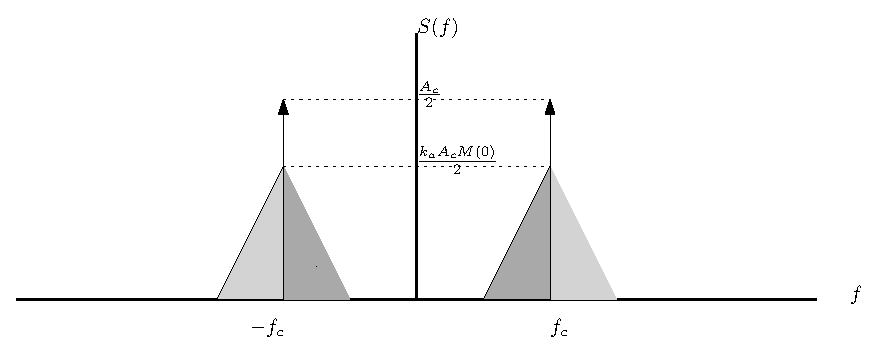
\includegraphics[scale=1]{chapters/chap01/images/mod.eps}
    \caption{Ilustração para equação \eqref{eq:mod_2}, adaptado de \cite{haykin2008}.}
\end{figure}

Pela equação \eqref{eq:mod_2}, observa-se que a parcela com impulsos unitários
não contribui diretamente para a transmissão da informação contida em $M(f)$,
além de despender grande parte da potência do sinal. Uma segunda característica
de $S(f)$ é a existência de dois lóbulos simétricos no domínio da
frequência, o que confere redundância na transmissão do sinal e maior largura de
banda. Para solucionar essas duas características indesejáveis em
telecomunicações, foram criadas as modulações com banda lateral dupla e
supressão de portadora (DSB-SC, do inglês \textit{double-sideband
suppressed-carrier}), banda lateral vestigial (VSB, do inglês \textit{vestigial
sideband modulation}) e banda lateral suprimida (SSB, do inglês
\textit{single-sideband modulation}), que vão além do escopo desse trabalho.

\abbrev{DSB-SC}{banda lateral dupla com supressão de portadora}
\abbrev{VSB}{banda lateral vestigial}
\abbrev{SSB}{banda lateral suprimida}

Uma notação mais simples para a equação \eqref{eq:mod_1}, presente na maior
parte da bibliografia, em que $k_a = 1$ e que desconsidera o \textit{offset}, é
dada pelo produto dos termos:
\begin{equation}
    s(t) = m(t)c(t). \label{eq:signal_eq}
\end{equation}
No domínio do tempo discreto,
\symbl{$m \lbrack n \rbrack$}{moduladora no domínio discreto}
\symbl{$c \lbrack n \rbrack$}{portadora no domínio discreto}
\symbl{$s \lbrack n \rbrack$}{sinal modulado no domínio discreto}
\begin{equation}
    s[n] = m[n]c[n]. 
\end{equation}

As parcelas moduladoras $m(t)$ e $m[n]$ podem assumir valores complexos
 \cite{schimmel2007}, apesar do termo \textit{envoltória} referir-se,
 geralmente, à parcela de valores reais não-negativos \cite{haykin2008} com
 lenta variação sobre um sinal. No caso particular em que $m(t)$ é um sinal de
 valores reais não-negativos, para a equação \eqref{eq:signal_eq}, temos que:

\begin{equation}
    m(t) \geq s(t), \forall t.
\end{equation}
A decomposição do sinal em envoltória e portadora em valores complexos é
abordada por \citet{atlas2004}.